\chapter{Development of a Reduced-Complexity Protein Representation and Coarse-Grained Build Strategy}
\label{chapter:reduced_rep}


\begin{quote}
``I have opinions of my own -- strong opinions -- but I don't always agree with them.'' \\
--- \textit{George Bush}
\end{quote}

\section{Introduction}

As has been discussed, the structure of globular proteins can be conceptually divided into regions of regular secondary structure, mainly \ahelixs\ and \bstrands, termed the protein-core and  loop-structures which connect them. The prediction of these loops remains the most taxing element of comparative modelling, largely due to the lack of homology information in the template structures for these regions. Generally, other than the primary sequence, the only information available to the modelling process is the location at which the loop enters and leaves the protein core. The conformational space, of loops greater in length than around seven residues, is not well represented by available PDB\ fragments. The structure of these longer loops must, therefore, be modelled using non-comparative methodologies.


The overall aim for this chapter is to describe the development of a torsional reduced-representation, coupled to a rapid method  for the enumeration  of conformational states and a complementary structural filtering procedure. The output of such a build-method is a list of   defined torsional states, which represent the available coarse-grained conformational space. This is an ideal foundation for a hierarchical torsional-refinement procedure, as large regions of conformational space may be eliminated from the more computationally costly refinement process. The development of the refinement levels is described in chapter \ref{chapter:prearcus}.
\section{Reducing Complexity}
\label{section:complexity}

The idea behind reduced protein representations has already been partially discussed in section \ref{section:protein_rep}. Studies have also been performed which look at the applications for reduced state models\cite{METHOD:Kol2004,METHOD:Sko98}. The central concept is that conformational space can be reduced to a large extent, without compromising the detail of the protein model. The reduction should be planned carefully to ensure that its ability to represent the native state is not  fundamentally impaired.
 
 When designing a reduced-representation a number of key choices are made. The first is the atomic representation, the second is how space will be described, third is the energy function that will discriminate between the states and finally some form of sampling mechanism must be chosen. The majority of reduced models utilise a much lower number of particles than would be contained within an all-atom model, for example using single-particle centroids positioned along the \ca$\to$\cb\ vector to represent the \sidechain\ atoms\cite{COMPCHEM:Gib2001}. The exact definition of the \forcefield\ is tightly-coupled to the chosen protein representation, because the shape of the energy wells has to take any simplified-geometry into account. 

Many different method developments have explored the discretisation of conformational space. Several have attempted to use lattice models, which simplify Cartesian space using discretised coordinate systems, at least for the \mainchain\ atoms in the model.  These lattice definitions include tetrahedral lattices\cite{COMPCHEM:Hin92},  extended face-centred cubic lattices\cite{METHOD:Cov90} and ``knights-walk'' lattices\cite{METHOD:Sko93}, with conformation counts of \mbox{$3^{n/2}-3$}, \mbox{$41^{n-3}$} and \mbox{$55^{n-3}$} respectively. At the crudest cubic-grid level, the representation is relatively poor, however, non-cubic fine-grid systems have been shown to approximate the native state of a protein to near-atomic accuracy\cite{METHOD:Kol2003}. Other methods, use continuous-space models with reduced degrees of freedom, for example some have used optimised limited sets of backbone torsion angles to represent the path of the protein chain\cite{COMPCHEM:Gib2001,COMPCHEM:Rooman91}. 

The central question is, how detailed does a reduced conformational representation need to be in order to represent the native conformation with sufficient accuracy? The results from a previous study \cite{METHOD:ParkLevitt}, which analysed the relationship between model-complexity and the accuracy of structural description, are shown in figure \ref{fig:reducedrep:complexity}. 

\begin{figure}[hbtp]
\begin{center}
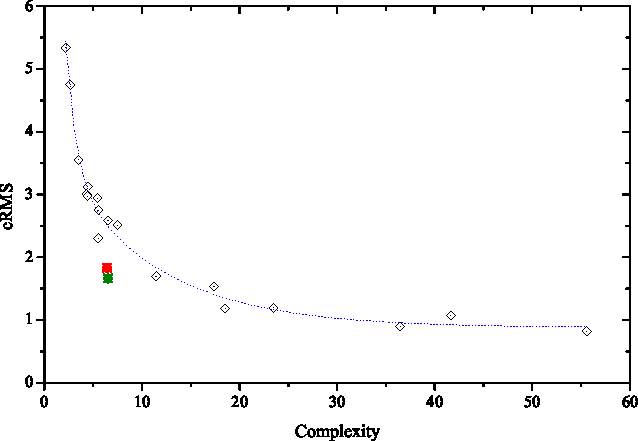
\includegraphics[width=0.85\textwidth]{./05-ReducedRep/complexity/complexity.pdf}
\caption[The relationship between model-complexity
and structural-representation]{The relationship between model-complexity
and structural-representation.\\
A fit is shown to a second-order exponential decay. Two representations are highlighted, which out-perform
the other methods in terms of finding an optimal balance between complexity and representation. These are the optimised torsional representations of Rooman et al.\cite{COMPCHEM:Rooman91}
and Park et al.\cite{METHOD:ParkLevitt} shown in red and green respectively.
(Data\cite{METHOD:ParkLevitt}.)}
\label{fig:reducedrep:complexity}
\end{center}
\end{figure}

Two broad trends are clear; The first is that as complexity increases, the quality of the representation
quickly plateaus to a cRMS of around 1.0\AA, signifying that overly-complex reduced representations yield no appreciable additional benefit. The second trend is that the representations which strike the best balance  are optimised torsional models. Further development of such a torsional representation is considered in this work, continuing from the published method 
\raft\cite{COMPCHEM:Gib2001}.
    
  
\section{The History of RAFT}

\raft\cite{COMPCHEM:Gib2001}, or Reduced Angle Forcefield for Tertiary structure prediction, was originally developed at the \uob,\ for application to \abinitio\ structure prediction of small protein molecules. The basic philosophy behind this implementation was to vastly reduce the scale of conformational space, by modelling the protein backbone with a limited set of residue-specific torsion-angle pairs, derived from PDB data.
As has been discussed, the reason that the conformational space of peptides can be reduced, is that the Ramachandran plot is limited to certain discrete areas of torsional space and reasonably compact in distribution. 

Six, residue-dependent \phipsi\ angle-pairs in three Ramachandran regions were allocated in the original \raft\ study. Two were defined to be typical $\alpha$-helical angles, three \bstrand\ angles and finally a single left-handed helical angle. 
For a given peptide, a series of these identifiers of the same length is termed a \emph{conformer}, which completely defines a given backbone conformation within the reduced set. The reduced \angleset\ was developed in combination with a simplified reduced-particle  forcefield for rapid energy evaluation of potential structures. 
Figure \ref{fig:reducedrep:raft_conformers} shows that, within this approximation, the ability to fold the native state is very reasonable for peptide fragments -- each example shown is proposed to be a small independent folding unit\cite{COMPCHEM:Ped1997}. 



\begin{figure}[hbtp]
\begin{center}
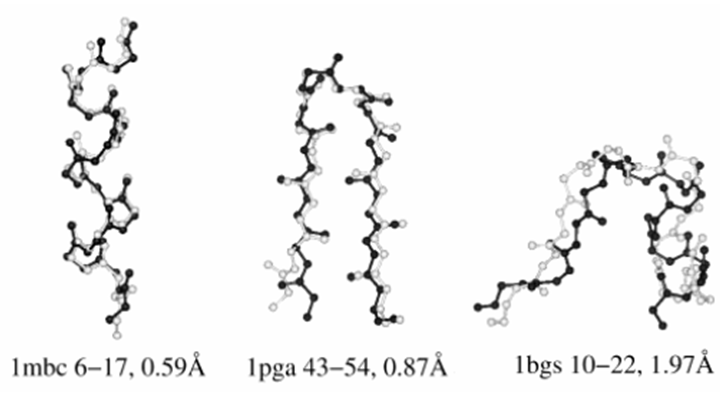
\includegraphics[width=0.67\textwidth]{05-ReducedRep/complexity/conformer.png}
\end{center}
\caption[Example \raft\ conformers]{Example \raft\ predictions. Each native peptide is proposed to be an independent folding-unit\cite{COMPCHEM:Ped1997}. The crystal-fragment and predicted structures are shown in black and grey respectively. The PDBID, residue range and \ca-cRMS appear below each image. Image adapted from\cite{COMPCHEM:Gib2001}.}
\label{fig:reducedrep:raft_conformers}
\end{figure}



\section{Six-state Loop-Modelling is Non-Trivial}

Modelling the conformation of a short surface loop may seem like an insignificant task, however, the difficulty becomes evident when the number of possible conformations which can be adopted is considered.  Assuming just six particular states and ignoring the conformational freedom of any \sidechains\, the exhaustive search on a \mer{12} loop yields 6\superscript{12} possible conformations -- \ie\ 2,176,782,336 structures in total. 

Of course, the majority of these conformers will not satisfy the restraints of entering and leaving the protein core at the correct locations and in the correct orientation. A significant proportion will also sterically clash with either themselves or with the protein surface. These facts are, however, not known from the outset and therefore building and subsequent evaluation of these conformations must be performed, before they can be eliminated from the search process. 

Following on from this idea, it is clear that full energetic evaluation of all potential loop structures would be hugely wasteful. Merely a 5 second building process and energy evaluation on each of these structures, for just one loop, would take a total of over 345 years. It is, therefore, clear that some sort of rapid culling of large numbers of conformations  is required, followed by effective sampling of the surrounding conformational space.

This process of culling potential loop structures can be relatively easily vocalised - simple statements like ``remove clashing conformations'' are easy to say - however the technical details of how one would efficiently perform this computationally is more complex. The computational practicality of storing coordinates for all these possible conformations or re-deriving the coordinates at every step is barely feasible -- just marking the viability of all conformations true or false for a given \mer{12} conformation in memory, each requiring just 1 bit, which would require 260\mb\ of storage; storing the energy would require 8.11\gb. Even at this level of storage, the need to convert valid bit-positions back into their conformers is ignored, but is required to facilitate sorting and subsequent re-evaluation under more complex calculations.
All-in-all, this describes the need for careful design of the computational method behind any build process to ensure tractability of the calculation.   



\section{Ramachandran Distributions}

Firstly, it is important to discuss the gross population distribution changes which occur when loop regions are considered in isolation. Three types of Ramachandran plot are shown in figure \ref{fig:reducedrep:ramachandran} to illustrate the different aspects. Glycine and proline are excluded from these plots due to large differences in their distributions and are discussed separately later in this chapter.

\begin{figure}[hbtp]
  \begin{center}
    \mbox{
      \subfigure[All structure scatter\superscript{1}]{\scalebox{0.42}{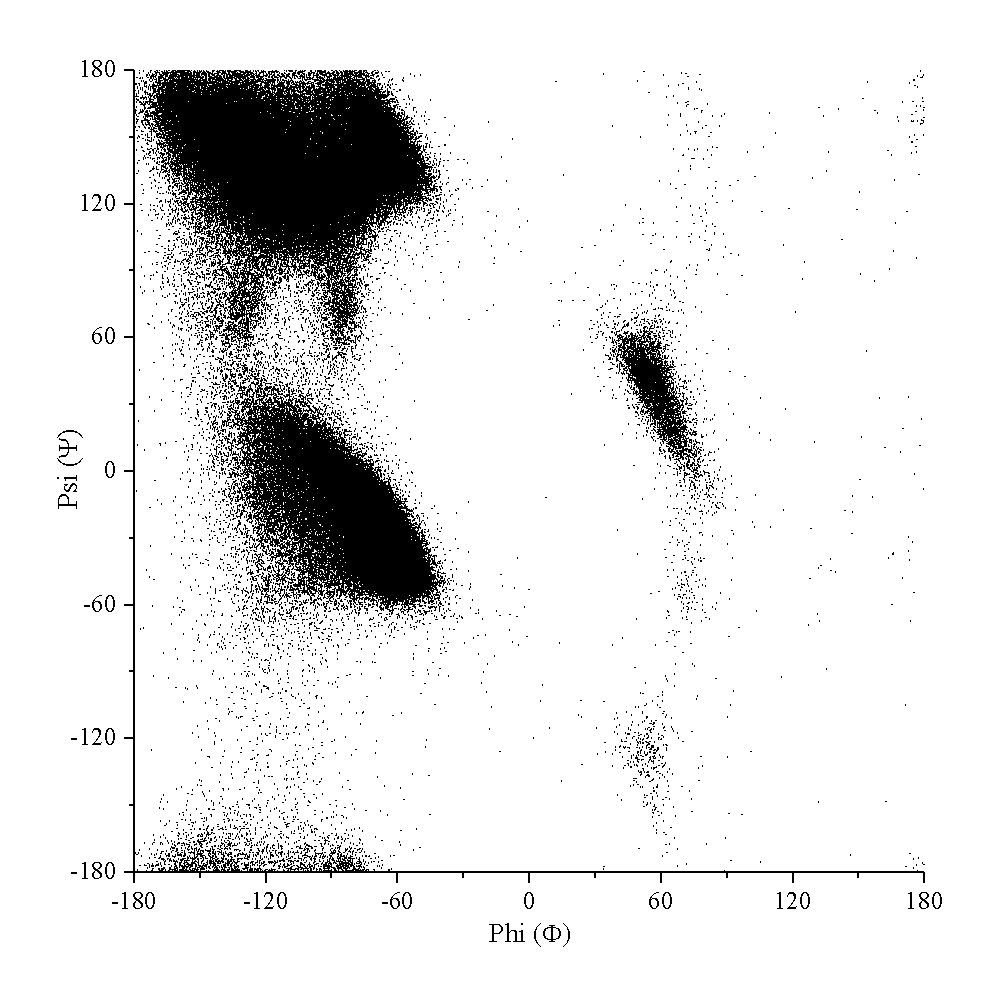
\includegraphics[width=1.0\textwidth]{05-ReducedRep/ram_plot/NotGlyOrPro_All_B_Scatter.png}}} \quad
      \subfigure[Loop structure scatter\superscript{2}]{\scalebox{0.42}{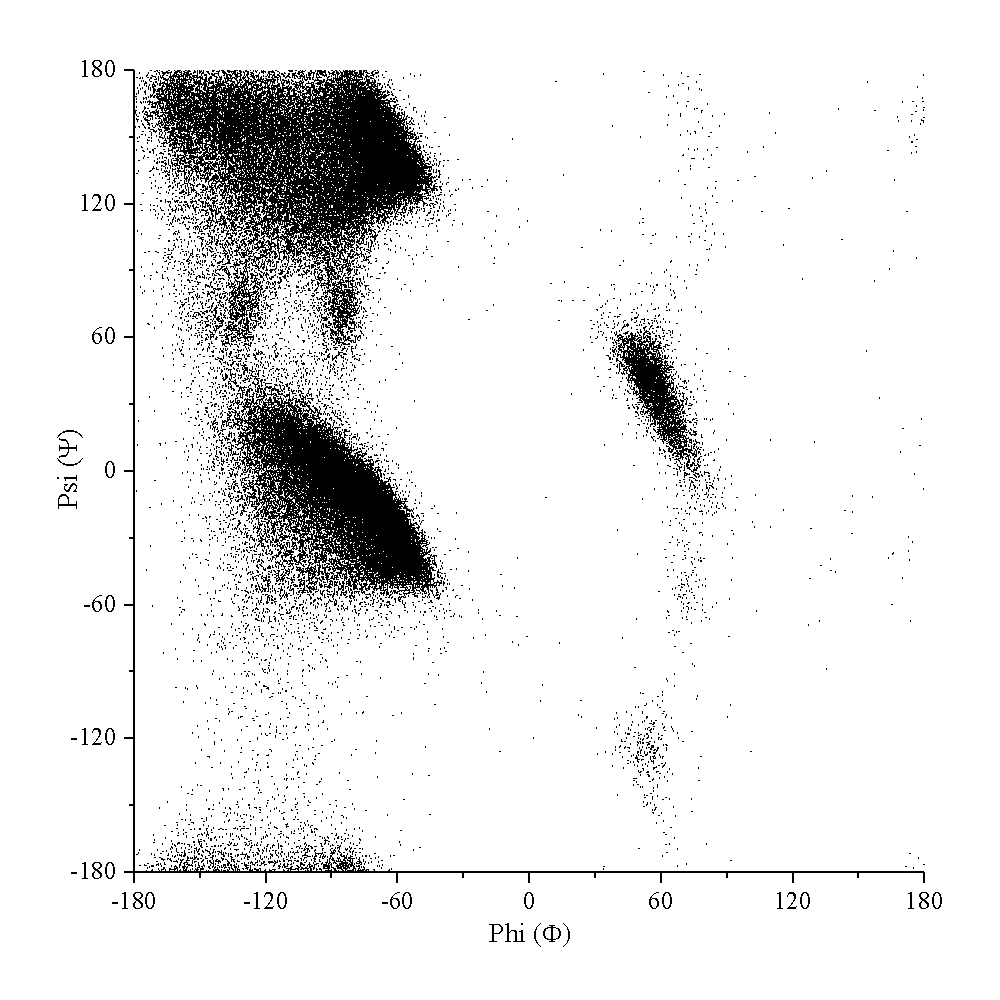
\includegraphics[width=1.0\textwidth]{05-ReducedRep/ram_plot/NotGlyOrPro_Loop_B_Scatter.png}}}
      }
      \vspace{0.5cm}
    \mbox{
      \subfigure[All structure 3D landscape\superscript{1}]{\scalebox{0.42}{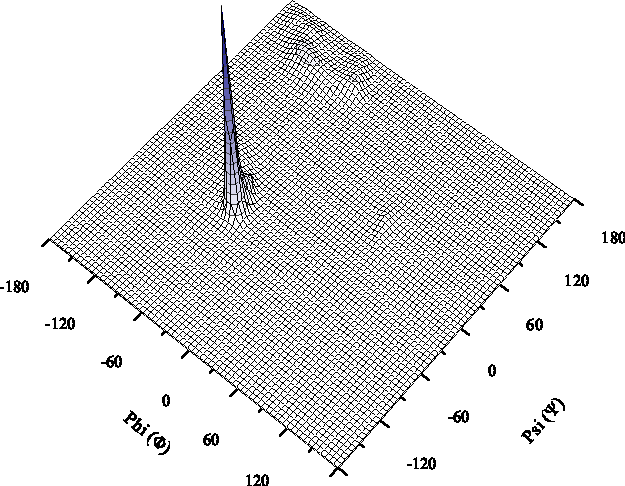
\includegraphics[width=1.0\textwidth]{05-ReducedRep/ram_plot/NotGlyOrPro_All_B_Contour3D.pdf}}} \quad
      \subfigure[Loop structure 3D landscape\superscript{2}]{\scalebox{0.42}{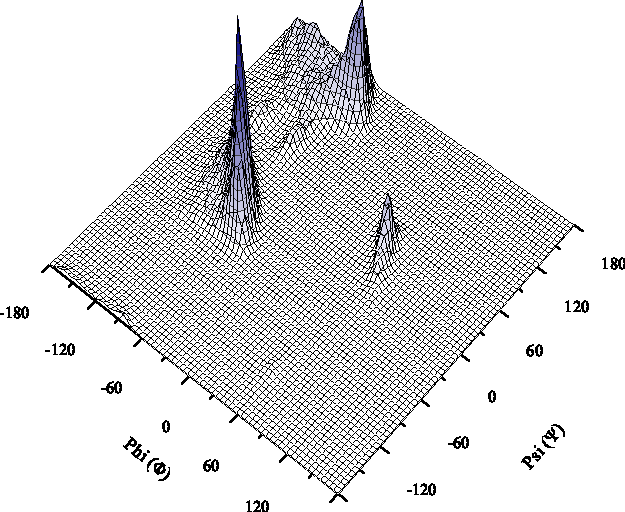
\includegraphics[width=1.0\textwidth]{05-ReducedRep/ram_plot/NotGlyOrPro_Loop_B_Contour3D.pdf}}}       }
      \vspace{0.5cm}
    \mbox{
      \subfigure[All structure contour\superscript{1}]{\scalebox{0.42}{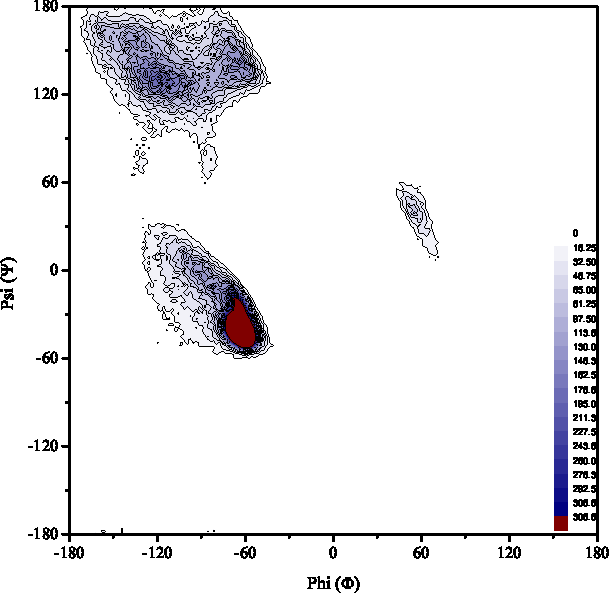
\includegraphics[width=1.0\textwidth]{05-ReducedRep/ram_plot/NotGlyOrPro_All_B_ContourHiRes.pdf}}} \quad
      \subfigure[Loop structure contour\superscript{2}]{\scalebox{0.42}{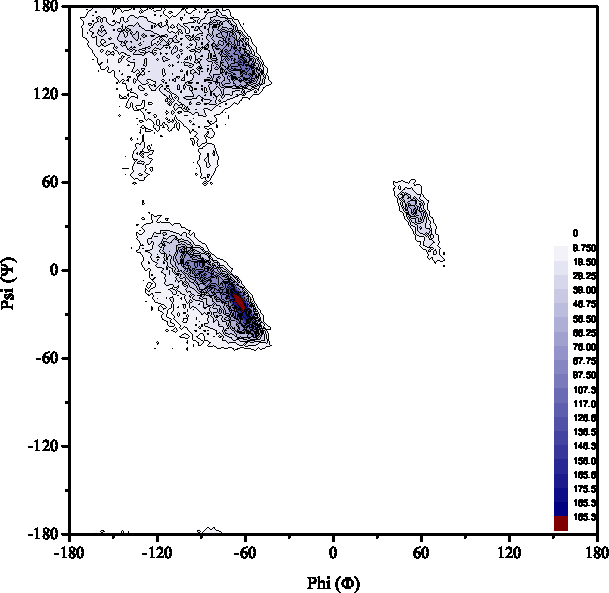
\includegraphics[width=1.0\textwidth]{05-ReducedRep/ram_plot/NotGlyOrPro_Loop_B_ContourHiRes.pdf}}}       }
\caption[Ramachanran distribution changes in loop regions]%
{Ramachandran distribution changes in loop regions. Data derived from all residue types except glycine and proline. Data\superscript{1}: 348,915 occurrences (87.74\%) in all structural classes. Data\superscript{2}: 130,147 occurrences (80.22\%) in loop structure only.}
    \label{fig:reducedrep:ramachandran}
  \end{center}
\end{figure}

The overall Ramachandran plot distribution remains unchanged when loop-structure is considered in isolation. This is to be expected, as the occupied regions of the Ramachandran plot are determined predominantly by steric interactions. Figure \ref{fig:reducedrep:ramachandran}-a, however, does show that the central density of the highly populated regions thins when only loops are considered, leaving proportionally more scattered data. From figure \ref{fig:reducedrep:ramachandran}-b it can be seen that the $\alpha$-region in globular protein structure is hugely favoured, reducing dramatically in loop regions as the helical bias is less pronounced. The change is shown quantitatively in figure \ref{fig:reduced_rep:propensity_change}.
Finally, in figure \ref{fig:reducedrep:ramachandran}-c it can be seen that the gross distribution within both the \al\ and \be-regions alters when loop regions are isolated.
When the \be-region for all structural data is considered, the population centred around  \mbox{$\Phi=$ -139, $\Psi=$ 135} is due to anti-parallel \bsheet. Evidently, the regularity of the anti-parallel \bsheet\ imposes conformational restrictions which are not present in loop structure, as there is a shift towards $\Phi=$ -70 in this case.

\begin{sidewaysfigure}[hptb]
\begin{center}
\subfigure[Angle-pair indices]{\scalebox{0.32}%
{
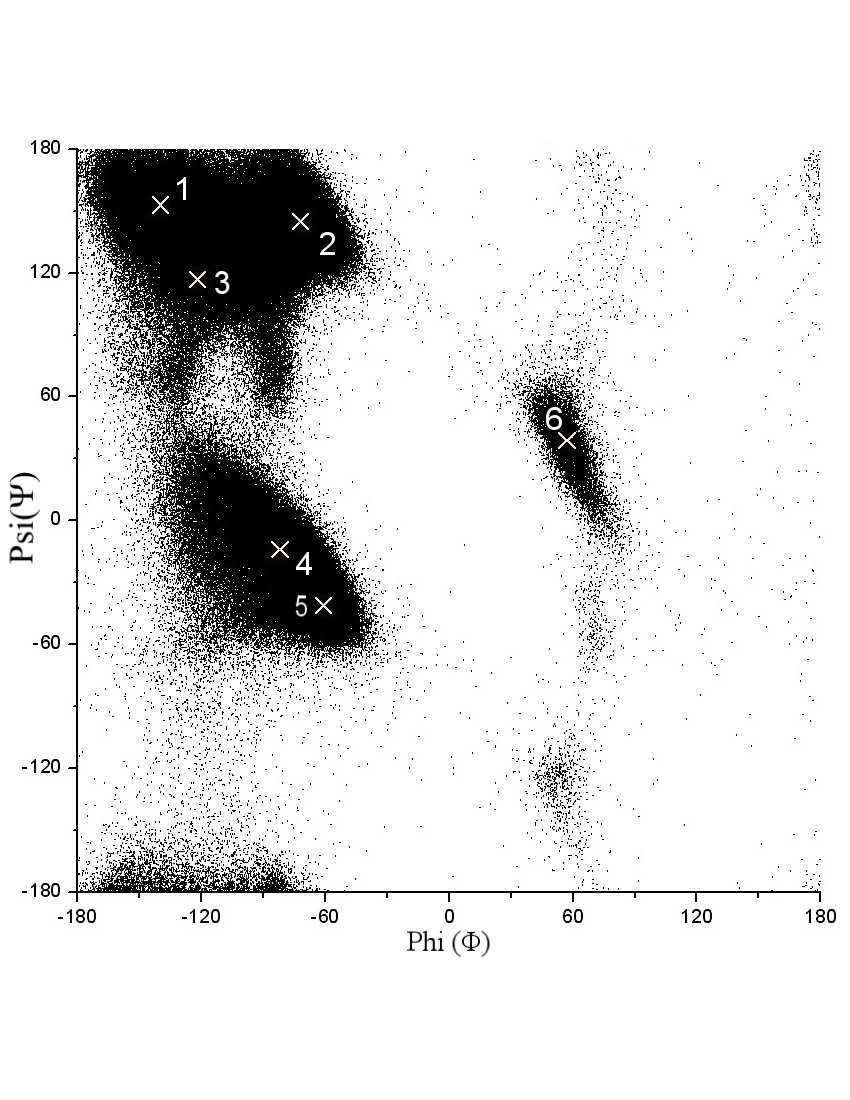
\includegraphics[width=1.0\textwidth]{05-ReducedRep/propensity/ramachandran.png} }}\qquad\subfigure[Comparing the \raft, all-structure and loop-structure \anglesets]{\scalebox{0.6}%
{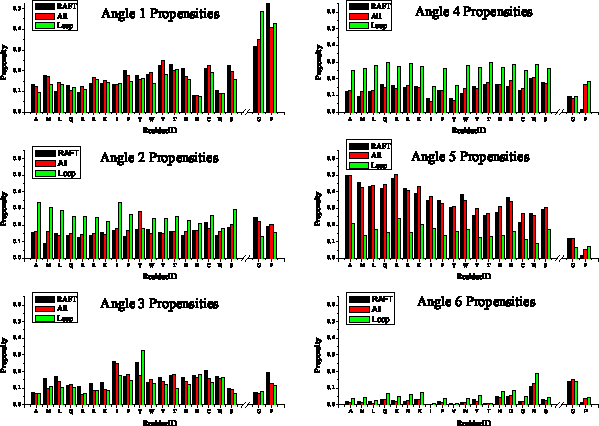
\includegraphics[width=1.0\textwidth]{05-ReducedRep/propensity/propensity.pdf}}}
\end{center}
\caption{Propensity changes between different structural classifications; when using six parametised angles.}
\label{fig:reduced_rep:propensity_change}
\end{sidewaysfigure}

\section{Structural Considerations}

We have described that the original \raft\ \angleset\ shows promise for small proteins and therefore, as the overall Ramachandran distribution does not change for loop regions, should be applicable to loop-modelling. We have, however, also shown that there is significant change in the relative distribution between Ramachandran regions when loops are considered in isolation. This implies that re-fitting should be performed to assess changes in optimal angle placement for loop regions, analyse whether more angles per-residue are required to account for increased variability and to measure the propensity for each angle-state.

\subsection{Glycine and Proline}

It is especially important to represent glycine and proline correctly in this study because they are more prevalent in loop regions by 157.5\% and 161.7\% respectively (table \ref{table:database:propensity}).
Due to the lack of \sidechain, glycine is less sterically hindered and can therefore routinely adopt backbone torsional angles that the other residues cannot. The six selected angles are therefore more diffuse in order to cover the required extra conformational space. A second special case, proline, is more conformationally restrained due to the fact that the \sidechain\ covalently bonds back onto its amino-group. This means that its $\Phi$-angle is largely inflexible resulting in a reduction in conformational diversity. Proline was originally fitted to two distributions on the Ramachandran map corresponding to the two predominant populations of the $\Psi$-angle. Specific aspects for both these residues are discussed as appropriate below.

\subsection{Backbone Stereochemistry}

Figure \ref{fig:intro:bb_torsion} was previously used to show that the protein \mainchain\ can be effectively described by three torsions per residue.
Relative occurrences of the cis and trans-peptide conformations were calculated during this work and are shown in  table \ref{table:intro:cis_occurence}. 
\begin{table}[htbp]
\begin{center}
\begin{tabular}{+l^r^r^r}
\toprule
\rowstyle{\bfseries} Type    &    Trans &  Cis  & \% Cis \\
\midrule
Proline &   32,591 & 1,960 &  5.67\% \\
Other  &   705,014 &   305 &  0.04\% \\
\bottomrule
\end{tabular}
\caption{Occurrences of the cis-peptide group conformation.}
\label{table:intro:cis_occurence}
\end{center}
\end{table}

Figure \ref{fig:reducedrep:omg}
shows that the conformational freedom of the  \Omg-torsion
is highly restricted in nature. Due to this 
inflexibility, the \Omg-torsion is commonly neglected in many modelling methods, treated exclusively as the trans-state. Compared to other residues, however, the \Omg-torsion of proline is an important consideration for modelling due to its  vastly increased occurrence as a  cis-peptide. In fact, the vast majority of cis-proline residues can be attributed to loop-structure in general. Due to this importance, the cis-state of proline is defined within the model used for this dissertation, but treated as a constant of either 180\degree\ or 0\degree\ for the build process alone. All other residues are treated as though they are in the trans-conformation.

\begin{figure}[htbp]
  \begin{center}
    \mbox{
      \subfigure[All Residues Except Proline]{
      \scalebox{0.45}{
      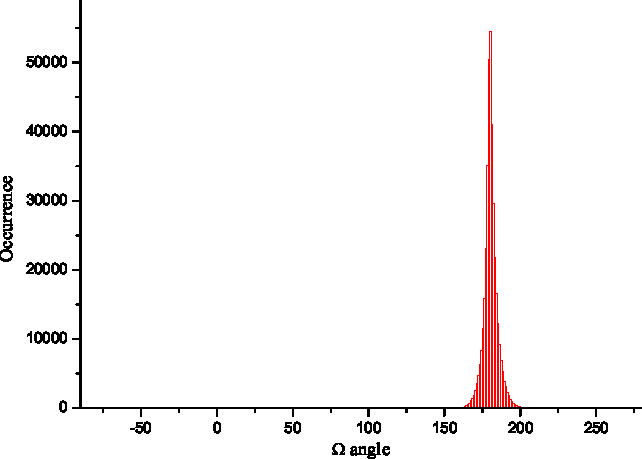
\includegraphics[width=1.0\textwidth]{05-ReducedRep/cis/omega_dist_allNoPro.pdf}}} \quad
      \subfigure[Proline]{
      \scalebox{0.45}{
      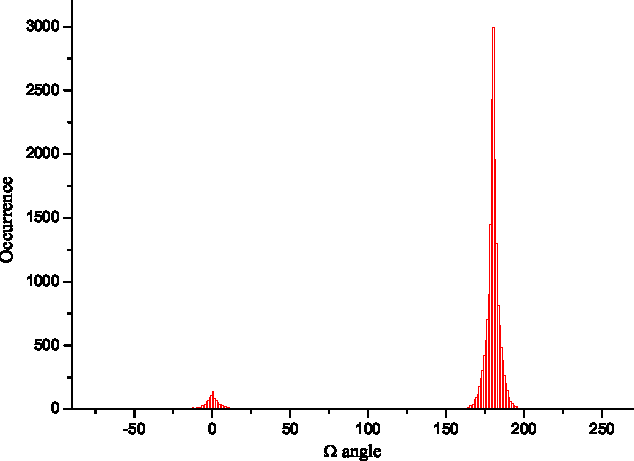
\includegraphics[width=1.0\textwidth]{05-ReducedRep/cis/omega_dist_proonly.pdf}}}
      }
    \caption{The distribution of the \Omg\ main-chain torsion.}
    \label{fig:reducedrep:omg}
  \end{center}
\end{figure}

It is noted that the remaining 305 non-proline cis-peptide occurrences are  highly important in the active sites of proteins and are, therefore, crucial to function. The neglect of the cis-state fundamentally means that the method developed in this work would  fail for these very rare specific cases. Such \Omg-angles could be enabled for short loops known to be part of an active-site, however, their general use is not feasible in terms of typical surface loop prediction. This is  both because the number of possible conformations is vastly increased and because the conformational search itself is polluted by large numbers of highly-improbable competing energy minima.


\subsection{Conformational Freedom vs. Angle-pair Count}

Figure \ref{fig:reducedrep:angle_coverage} shows that individual residue types are represented to different accuracies by six residue-states.
 In contrast to the original \raft\ study, which used six angles for every residue type, there is no reason why the number of angles cannot be varied on a per-residue basis. 
\begin{figure}[hbtp]
\begin{center}
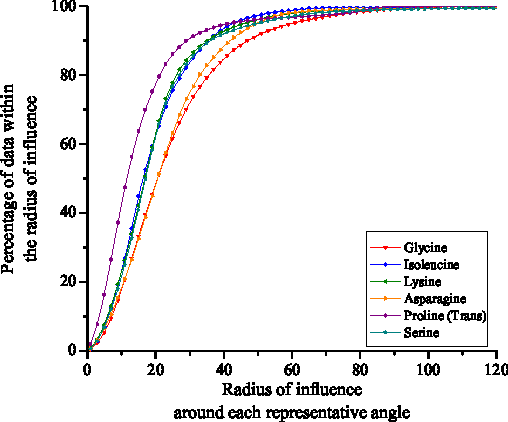
\includegraphics[width=0.7\textwidth]{05-ReducedRep/closest_angle/closest.pdf}
\caption[The data coverage of the original \raft\ \angleset.]{The data coverage of the original \raft\ \angleset. To obtain this plot, the relevant Ramachandran scatter-plot  is loaded per residue-type, with the matching representative \raft\ angle-pairs superimposed. Around each angle-pair, a circle is drawn. The radius of each circle is gradually increased and the percentage of data within all circles is measured at each increase. This radius is termed the radius of influence. In real terms this radius equates to the search radius which must be employed to generate the exact native loop conformation for a given percentage of native loops -- obtained via optimal torsional perturbations of \emph{up to} that magnitude.}
\label{fig:reducedrep:angle_coverage}
\end{center}
\end{figure}

A second aspect is one of implementation. Proline only required four parametised angles in the original \raft\ work, however it was given six angles purely to aid implementation of the software; Due to enhanced memory management of more modern software development platforms, shortcuts like this are no longer required. 

There are multiple cases which may need additional angles; serine occurs most regularly in the disallowed regions of the Ramachandran plot, glycine shows a vastly increased conformational spread and asparagine fits relatively poorly to  six residue-states.
Having specified a possible  need for additional angles when modelling loop regions, it should be emphasised that the converse argument is also true -- \ie although one could add many additional angles to give a fine-grained definition of conformational space, the huge problem of the ``conformational explosion'' must always be considered. For example, when exhaustively  enumerating the conformer for a typical \mer{12} fragment, increasing from a six-state \angleset\ to a seven-state \angleset\ yields 6.3$\times$ more conformers. Alternatively, by increasing to an eight-state \angleset, an increase of 31.6$\times$ occurs. This obviously increases a 1 day calculation to a 1 week and 1 month calculation respectively. This is not a cheap price to pay, especially when method calibration and parametisation is required and computational resources are limited. It should be remembered however that, as described in section \ref{section:complexity}, some modern lattice methods use conformational spaces which scale with $41^{n-3}$ or $55^{n-3}$, far in excess of the $6n$ of the original \raft\ study.


\subsection{Subsequent Refinement}
\label{section:reduced_rep:subsequentrefinement}

Figure \ref{fig:reducedrep:searchradius} shows that, under the original \raft\ angle-pair definitions, with respect to a second-stage torsional perturbation remodelling method, a 60\degree\ maximal perturbation would yield excellent data coverage.
One small caveat is that,
even perturbations of up to 120\degree\ would not cover the data within disallowed clusters II and III. These clusters are important for the $i+1$ position of some types of $\beta$-turn, as previously shown together to be important in up to 7\% of loops in table \ref{table:db:disallowedloop}. However, a search radius of 120\degree\ would not be computationally tractable in  later refinement stages.
As serine is known to occupy these regions with significant frequency, there is an argument for re-parametisation of this residue and possibly more fitted angle-pairs. It would be hoped that any automatic re-parametisation of angle-pairs for surface loop modelling would yield coverage of these regions for serine. 

\begin{figure}[hbtp]
\begin{center}
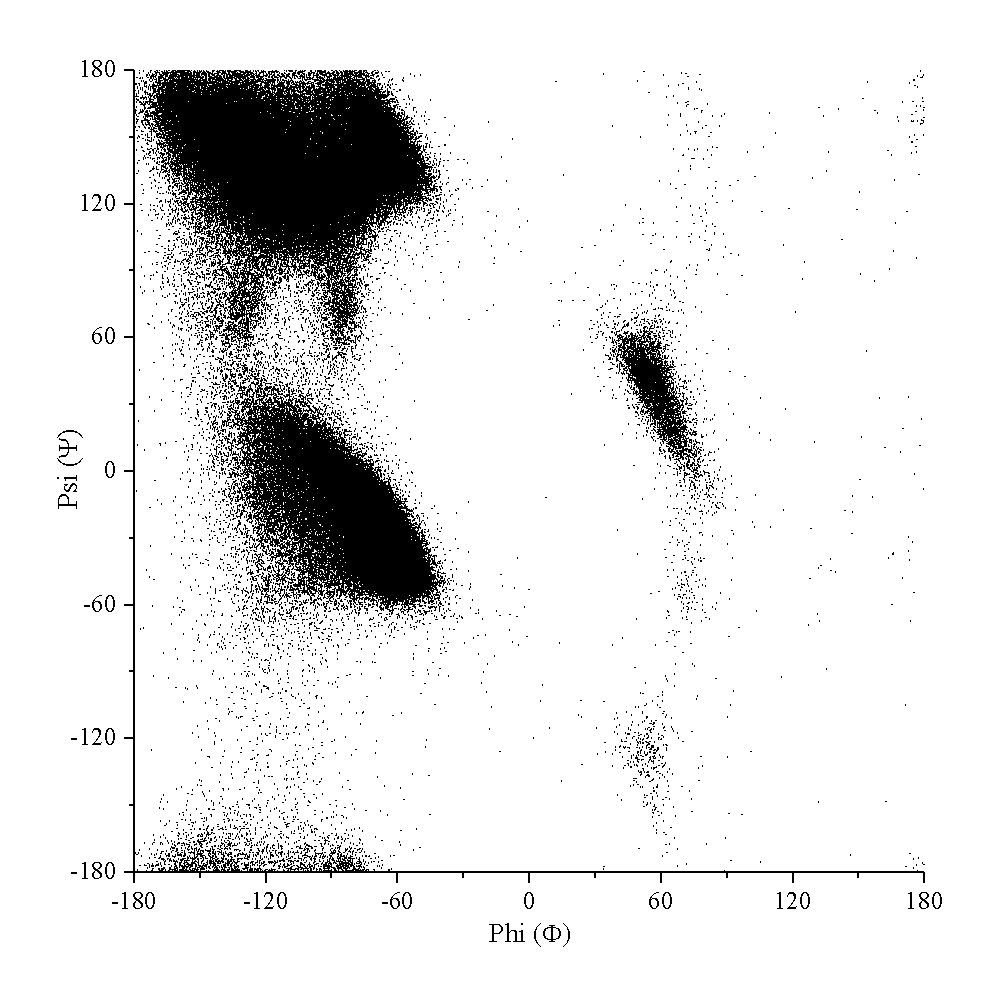
\includegraphics[width=0.55\textwidth]{05-ReducedRep/ram_plot/NotGlyOrPro_All_B_Scatter.png}
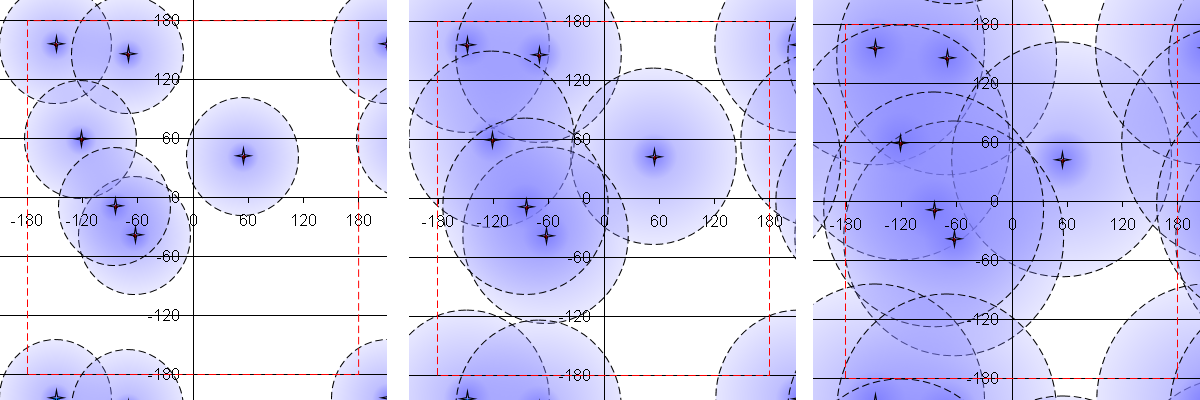
\includegraphics[width=0.95\textwidth]{05-ReducedRep/search/radius.png}
\caption[Torsional Search Radius]{%
Torsional search-radius.
An arbitrary set of six \raft\ angle-pairs are shown as stars, with $\pm$180\degree\ Ramachandran plot boundaries shown as red dashed lines. From left to right the radii of influence around the idealised angles are shown at 60\degree, 90\degree\ and 120\degree\ respectively.}
\label{fig:reducedrep:searchradius}
\end{center}
\end{figure}


\section{The Angle-fitting Method}

The fitting method in the original \raft\ study, was based on a 2D search of the Ramachandran plot, in order to minimise the total distance of all the data points to their nearest parametised angle. This essentially results in the representative angles being assigned to the most densely populated regions of the Ramachandran map. The scoring method has been kept in this study with one change, outlined below.

The fitting procedure was performed for each residue-type in isolation. Due to computational limitations, the original study used a course 1.0\degree\ grid, restricted to each of the three most populated Ramachandran regions. Following an exhaustive search over the three independent grids, a search using a smaller, finer 0.2\degree\ grid was performed for each allocated angle in turn. The solution obtained was the optimum for a given grid definition, however, intrinsically dependent on the arbitrary rectangular 2D boundaries chosen by the user. 

 An alternative procedure was chosen for this work as a scheme of random perturbations followed by the \emph{simultaneous} score minimisation for all fitted angle-pairs under the \raft\ scoring function.  In an iterative process, the $n$ angles were first placed in a random location on the Ramachandran plot,  followed by successive small-steps down the numerically-calculated score-gradient. To define the gradient, each \thothloopdb -derived data point was given a score equal to the square of the current distance to its closest parametised angle.
These distances were summed and the square-root taken. The minimisation was repeated until the score gradient reached zero; defining a local minimum. The entire procedure was then repeated until the score for 30 successive iterations did not improve. The value 30 is completely arbitrary, representing a conservatively high value based upon multiple independent test runs. The best converged solution found was then assumed to be the global minimum. This procedure has the intrinsic advantage of having no human-defined data boundaries and is not limited a coarse-grid search. This theoretically results in a better representation of the available data. Table \ref{table:reducedrep:anglefitting} shows that this method is robust and reaches convergence, to at least 0.1\degree\ from multiple independent runs.
All final \anglesets\ were also visually checked.

\begin{table}[hbtp]
\begin{small}
\begin{center}
\begin{tabular}{+l^r^r^r^r^r^r^r^r}
\toprule
\rowstyle{\bfseries}
  Angle     &  \multicolumn{2}{c}{Run 1} & \multicolumn{2}{c}{Run 2} & \multicolumn{2}{c}{Run 3}  & \multicolumn{2}{c}{Run 4} \\
\rowstyle{\bfseries}
  Index &  \multicolumn{1}{c}{$\Phi$}  &  \multicolumn{1}{c}{$\Psi$}  &  \multicolumn{1}{c}{$\Phi$}  &  \multicolumn{1}{c}{$\Psi$}  &  \multicolumn{1}{c}{$\Phi$}  &  \multicolumn{1}{c}{$\Psi$}  &  \multicolumn{1}{c}{$\Phi$}  &  \multicolumn{1}{c}{$\Psi$} \\
\midrule
  1  &  -65.15  &  -37.32  &  -65.14  &  -37.28  &  -65.14  &  -37.31  &  -65.12  &  -37.30 \\
  2  &  -143.18  &  164.65  &  -143.19  &  164.64  &  -143.25  &  164.67  &  -143.19  &  164.66 \\
  3  &  -106.56  &  101.41  &  -106.55  &  101.39  &  -106.56  &  101.41  &  -106.56  &  101.39 \\
  4  &  -72.66  &  145.45  &  -72.66  &  145.45  &  -72.67  &  145.43  &  -72.65  &  145.42 \\
  5  &  -97.76  &  4.32  &  -97.75  &  4.31  &  -97.76  &  4.34  &  -97.74  &  4.32 \\
  6  &  58.30  &  36.76  &  58.28  &  36.77  &  58.31  &  36.76  &  58.30  &  36.76 \\
\midrule
  Score  &  \multicolumn{2}{r}{25,918,937}  &  \multicolumn{2}{r}{25,918,944}  &  \multicolumn{2}{r}{25,918,946}  &  \multicolumn{2}{r}{25,918,948} \\
\bottomrule
\end{tabular}
\caption{Typical deviations in angle-pair parametisation from four identical fitting runs for aspartic acid.}
\label{table:reducedrep:anglefitting}
\end{center}
\end{small}
\end{table}

Two separate modes of angle-fitting were assessed. As a ``sanity check'' the search method used in this study was tested in combination with the three human-defined Ramachandran regions of the original \raft\ study. If the methods are comparable and the database used equally representative, then a very similar answer should be obtained for the same residue-type. This was found to be the case and therefore will not be discussed here further. 

\subsection{Propensity Derivation}

Following the parametisation of each angle-pair, it is desirable to obtain propensity for information. To calculate this information, each data-point is assigned to its closest parametised angle-pair, then the fraction of data covered calculated for each pair.
Obviously, the more data that is covered by a given pair, the more probable it is for that pair to occur within a randomly selected native loop structure.
\subsection{Implementation}

In order to implement the fitting procedure, the core assembly (section \ref{section:software:uob:core_assembly}) of the \uobf\ (section \ref{section:software:uob}) was used, in combination with \thothloopdb\ (section \ref{section:intro:loop_db}), to produce a specialised executable application. The role of this executable was both to perform the torsion-fitting procedure itself and to produce \angleset\ definition files for use with a complementary \angleset\ reader implemented in \pd\ (section \ref{section:software:pd}).
The final \angleset \ definition files themselves are presented in appendix \ref{appendix:angleset}.
A simple \angleset\ viewer was also produced to allow visualisation of each \angleset\ during testing.

\subsection{An Additional Consideration}

A feature of the scoring system used to fit angle-pairs for this work is that, if a single angle is required to represent two separated areas of density, it will be placed in between them in an area with little or no density.
The angle-pair itself is therefore not representative of the properties of the 3D system. In real terms, this occurs primarily for the lowest-propensity \be-angle, which resides between the two ``lobes'' that extend out below the \be-region.
This prompts the question of whether this is a desirable effect. 

Firstly, it is certainly undesirable to add too many additional angles as this exponentially increases the total number of possible conformations.  One option would be to pick one of the regions of density and neglect the second, however, this means that the neglected region will not be explored by the stage 2 refinement process. The decision of which region to occupy should, therefore, be left to the stage 2 refinement process itself.
Stage 2 by definition will employ more complex torsional energetic calculations that are non-discretised in nature. This algorithm is therefore better-placed to make the choice between the competing locally populated regions via perturbation and energetic minimisation in the three spatial dimensions.
So, from the perspective of this work, when required due to a limited number of angle-pairs, the occupation of such an unpopulated region in 2D space\ \emph{is} desirable.


\section{Fitting Results for \mer{6} to \mer{10} Angle-sets}

In the following section the results from the new angle-fitting procedure are analysed in relation to six residue case-studies as follows:

\begin{itemize} \isep
\item Lysine will be used as the residue which embodies the typical distribution of most residues; other examples in this class are: K, A, C, E, F, H, L, M, Q, R, W, Y.
\item   Isoleucine will be used as an example of a poorly populated left-handed helical region where fitting is divergent from that in the \raft\ study; other examples are: I, T, V.
These residues are the \be-branched residues, where the left-handed helical conformation is sterically hindered.\item    Asparagine is used as an example of a residue which shows an atypical $\beta$-region, categorised by a more diffuse distribution in the lower $\Phi$=90 region.
The other example is D. In general these differences are caused by the ability of the \sidechain\ to make hydrogen bonding contacts with the \mainchain.
\item   Serine is shown as a special case, as it is the residue which most often populates disallowed regions.
\item   Glycine is shown as it is a special residue exhibiting a larger dispersed data distribution.\item Proline  is shown as it is a uniquely constrained residue and therefore is the only residue which requires less than six angle-pairs.
\end{itemize}

For each case study, a figure is presented which is composed of  six cells. The first is used to show a 3D Ramachandran distribution for that residue-type. The remaining cells sequentially show between six and ten fitted angle-pairs, superimposed on the scatter plot. Each Ramachandran plot is composed only of data from loop regions. Proline is shown slightly differently, as the fitting process considered both the cis and trans-states and only fitted between two and six angle-pairs.  The points fitted to this data  should, therefore, correlate extremely well to the scatter density, if  valid. 

For each figure, the original six \raft\  angle-pairs are shown with both the angle-pairs derived in this study for all-structure-types and loop-structure only -- using black, red and green data-points respectively. The results from \raft\ and this work are in good agreement for six angle-pairs. Significant deviations can be seen for all residue-types when loop regions are considered in isolation. 

% -----------------------------------------------------
% As biig as possible withough causing float overflow
\newcommand{\anglesetscale}{0.444}
% -----------------------------------------------------

\subsection{Lysine: A Typical Distribution}

Lysine is shown here in figure \ref{fig:reducedrep:ramachandran:lys} to illustrate the trends seen following angle-fitting to the data for most residue types. The fitted angle-pairs closely represent the data-density in all sub-figures. Reassuringly, the human decision in the original \raft\ study is mirrored by the automated process in that three angles are given to the \be-region, two to the \al-region and one to the left-handed helical region.\ As expected, the angle at around $\Phi$=120 $\Psi$=-110 covers the diffuse distribution of the data in the lower \be-region. 

When six-angles are fitted to loop-structure data in figure \ref{fig:reducedrep:ramachandran:lys}-b, this fitted \be-angle drops to around $\Phi$=100, in order to better cover the two ``lobes'' that extend from the bottom of the \be-distribution; a trend which is seen for almost all of the amino acids. Interestingly when the fit is extended to seven angles in figure \ref{fig:reducedrep:ramachandran:lys}-c,  disallowed cluster II is then fitted for the both all-structure and loop-only fitting procedures, signifying its importance.
Additional angles beyond seven are then utilised in a better representation of the spread around the \al\ and \be-regions.
The precise allocation of these angles is dependent both on residue-type and whether all-structure or loop-structure is considered. The left-handed helical region is only given one angle in all cases, due to its tight distribution.

\begin{figure}[htbp]
  \begin{center}
    \mbox{
      \subfigure[3D Ramachandran distribution]{\scalebox{\anglesetscale}%
      {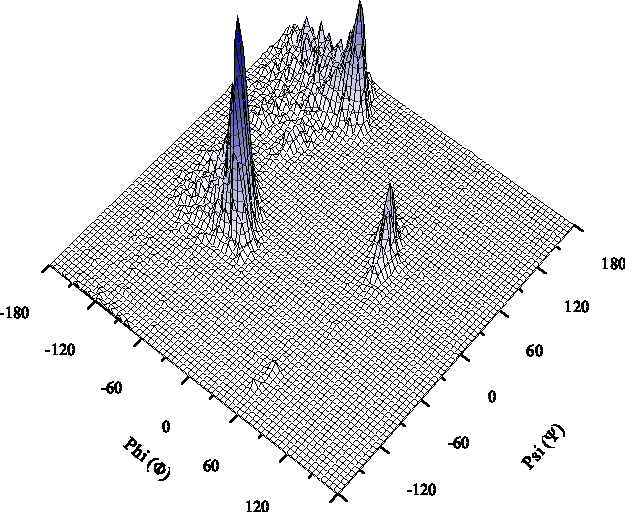
\includegraphics[width=1.0\textwidth]{05-ReducedRep/lysine/KT_Loop_B_Contour3D.pdf}}} \quad
      \subfigure[6 angle allocations]{\scalebox{\anglesetscale}%
      {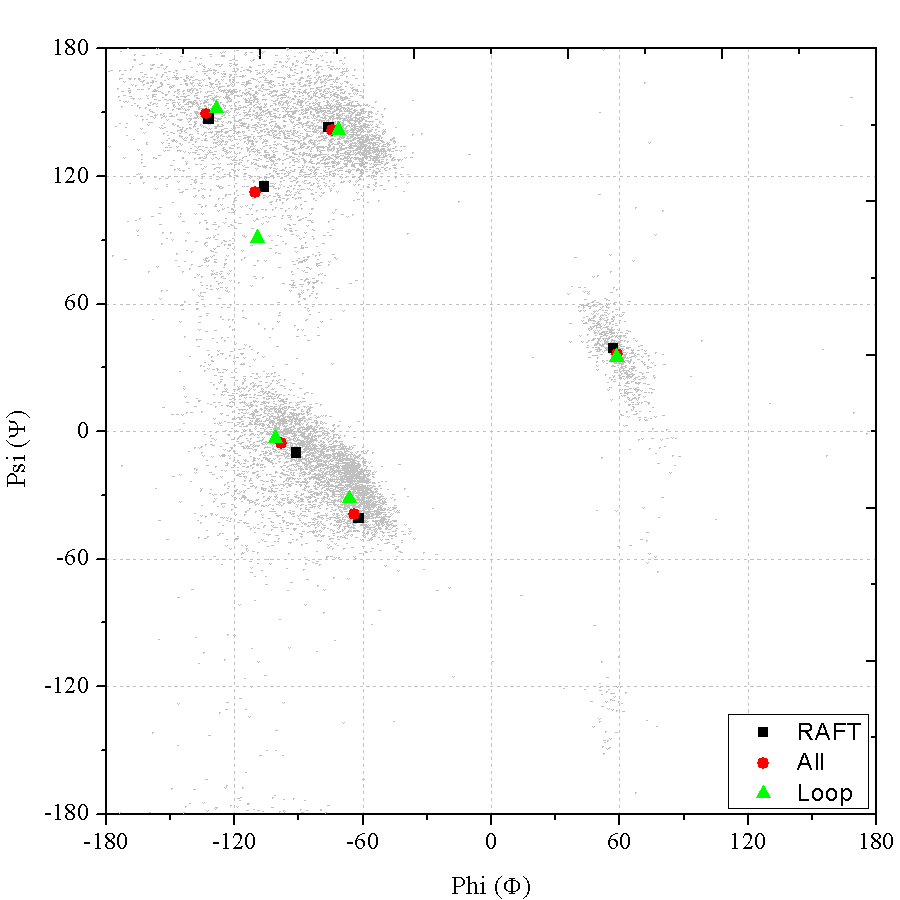
\includegraphics[width=1.0\textwidth]{05-ReducedRep/lysine/K_6_0_B_fitgraph.png}}}
      }
    \mbox{
      \subfigure[7 angle allocations]{\scalebox{\anglesetscale}%
      {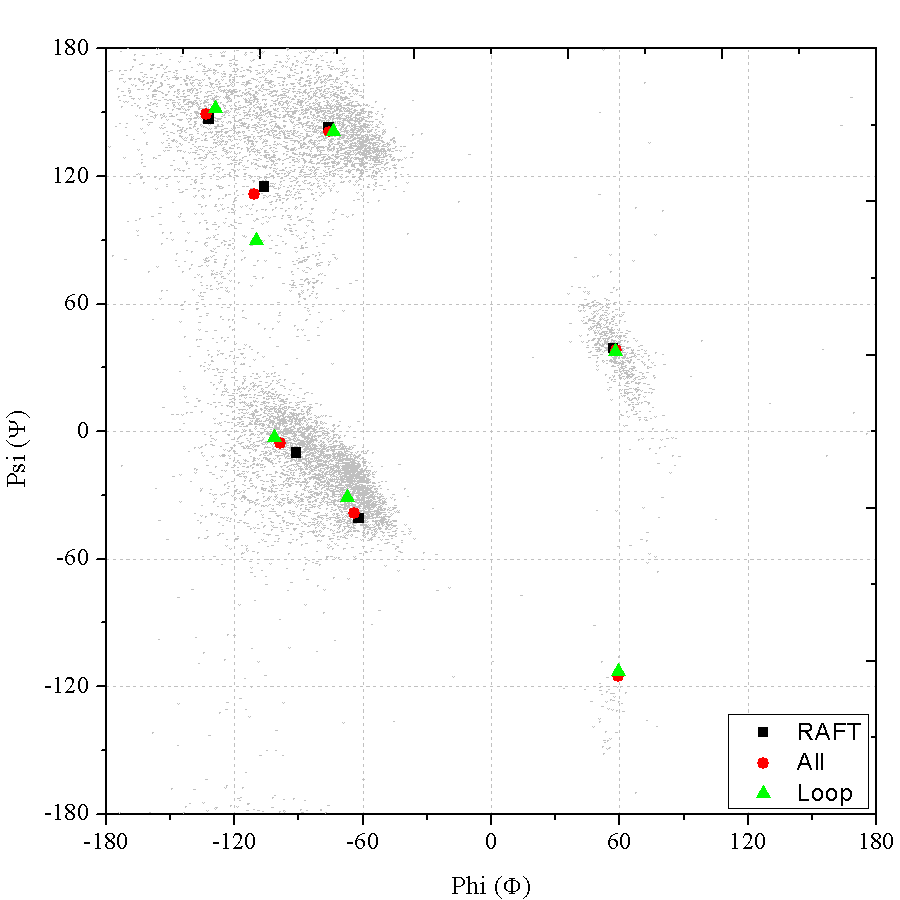
\includegraphics[width=1.0\textwidth]{05-ReducedRep/lysine/K_7_0_B_fitgraph.png}}} \quad
      \subfigure[8 angle allocations]{\scalebox{\anglesetscale}%
      {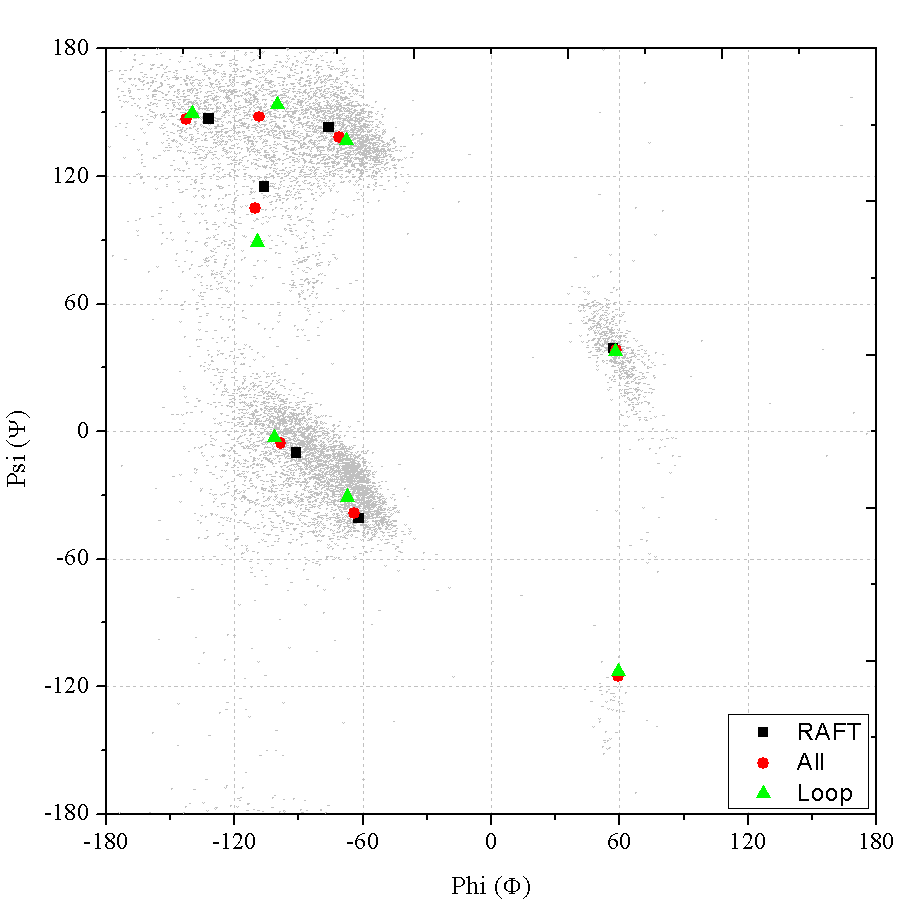
\includegraphics[width=1.0\textwidth]{05-ReducedRep/lysine/K_8_0_B_fitgraph.png}}}       }
    \mbox{
      \subfigure[9 angle allocations]{\scalebox{\anglesetscale}%
      {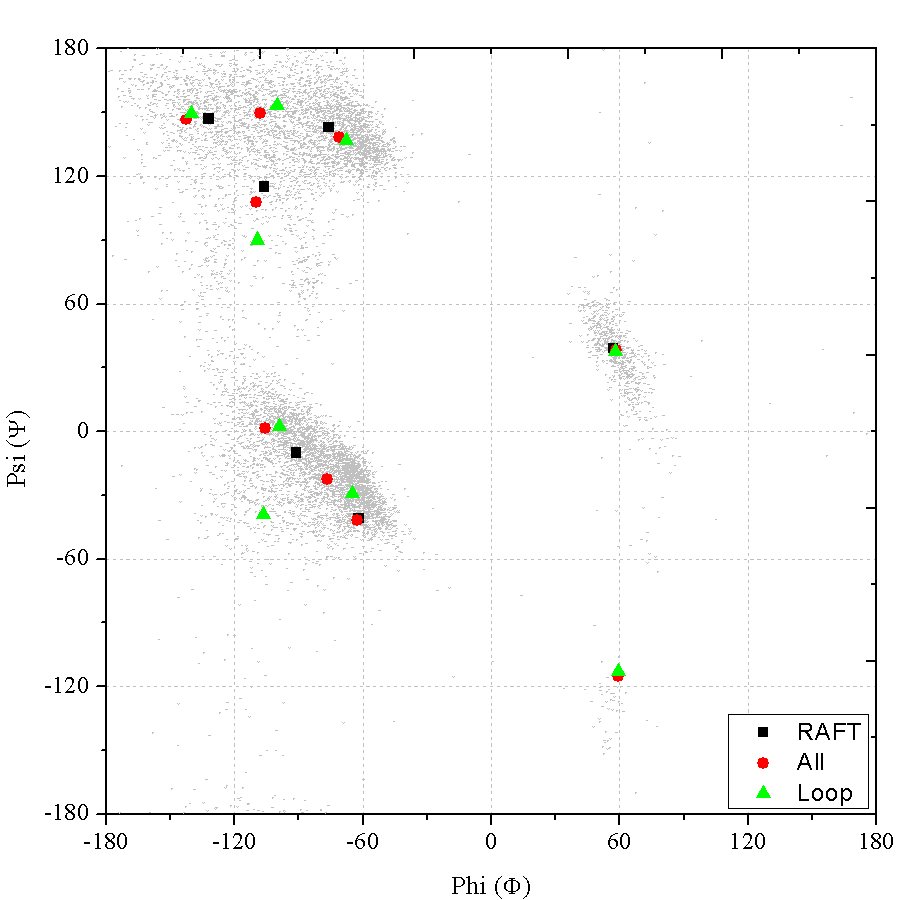
\includegraphics[width=1.0\textwidth]{05-ReducedRep/lysine/K_9_0_B_fitgraph.png}}} \quad
      \subfigure[10 angle allocations]{\scalebox{\anglesetscale}%
      {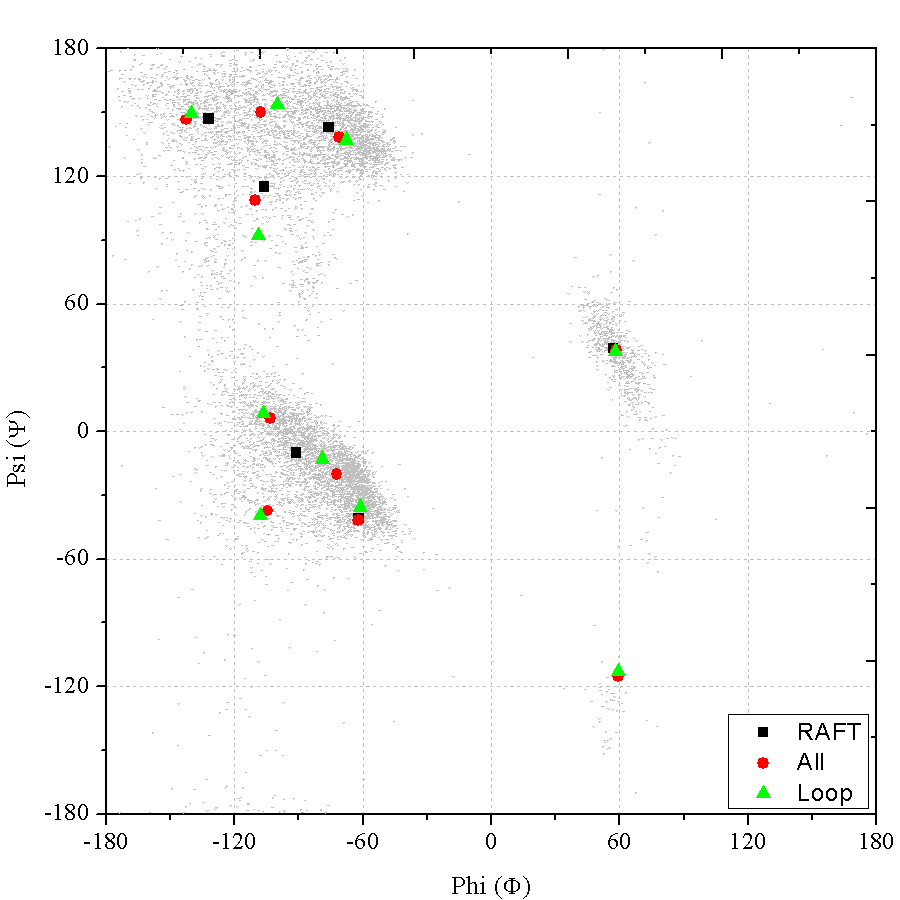
\includegraphics[width=1.0\textwidth]{05-ReducedRep/lysine/K_10_0_B_fitgraph.png}}}       }
\caption[Ramachanran distribution and angle fitting for lysine]%
{Ramachandran distribution and angle fitting for lysine.
Data: 9,342 occurrences (5.76\%) in loop regions only.}
    \label{fig:reducedrep:ramachandran:lys}
  \end{center}
\end{figure}


\subsection{Isoleucine: Sparse left-handed Helical Distribution}

As shown in figure \ref{fig:reducedrep:ramachandran:ile}, residues like isoleucine display a particularly low propensity for the left-handed helical region of the Ramachandran plot. In fact, in the case of isoleucine disallowed region II is equally populated, if not more so. In the original \raft\ study the angle-fitting grids were manually fixed in the three main regions of the plot in distinct user-specified regions. In this study where points are allowed to fit to any region of the plot the placement is not in agreement. In figure \ref{fig:reducedrep:ramachandran:ile}-b, the left-helical angle shifts from $\Phi$=30 to $\Phi$=0, pulled down by the distribution of points in the $\Phi$=-60 region, a trend that continues for 7 and 8 angle-pairs. For 9 angle-pair allocations or more, the disallowed region II cluster is represented by an angle and the left-handed helical angle-pair shifts up closer to that fitted by the original raft study.
Interestingly, in figure \ref{fig:reducedrep:ramachandran:ile}, the \xth{7} angle-pair allocation is utilised by the all-structure and loop-only sets in different ways. The loop-only fit chooses an additional angle for the \al-region, whereas the all-structure fit allocates an additional \be-angle. The decision is reversed when a further angle is added in figure \ref{fig:reducedrep:ramachandran:ile}-d.

\begin{figure}[htbp]
  \begin{center}
    \mbox{
      \subfigure[Ramachandran distribution]{\scalebox{\anglesetscale}%
      {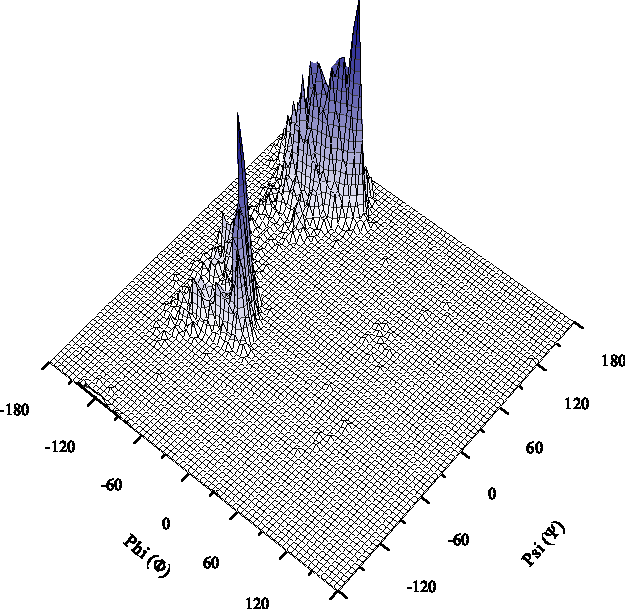
\includegraphics[width=1.0\textwidth]{05-ReducedRep/isoleucine/IT_Loop_B_Contour3D.pdf}}} \quad
      \subfigure[6 angle allocations]{\scalebox{\anglesetscale}%
      {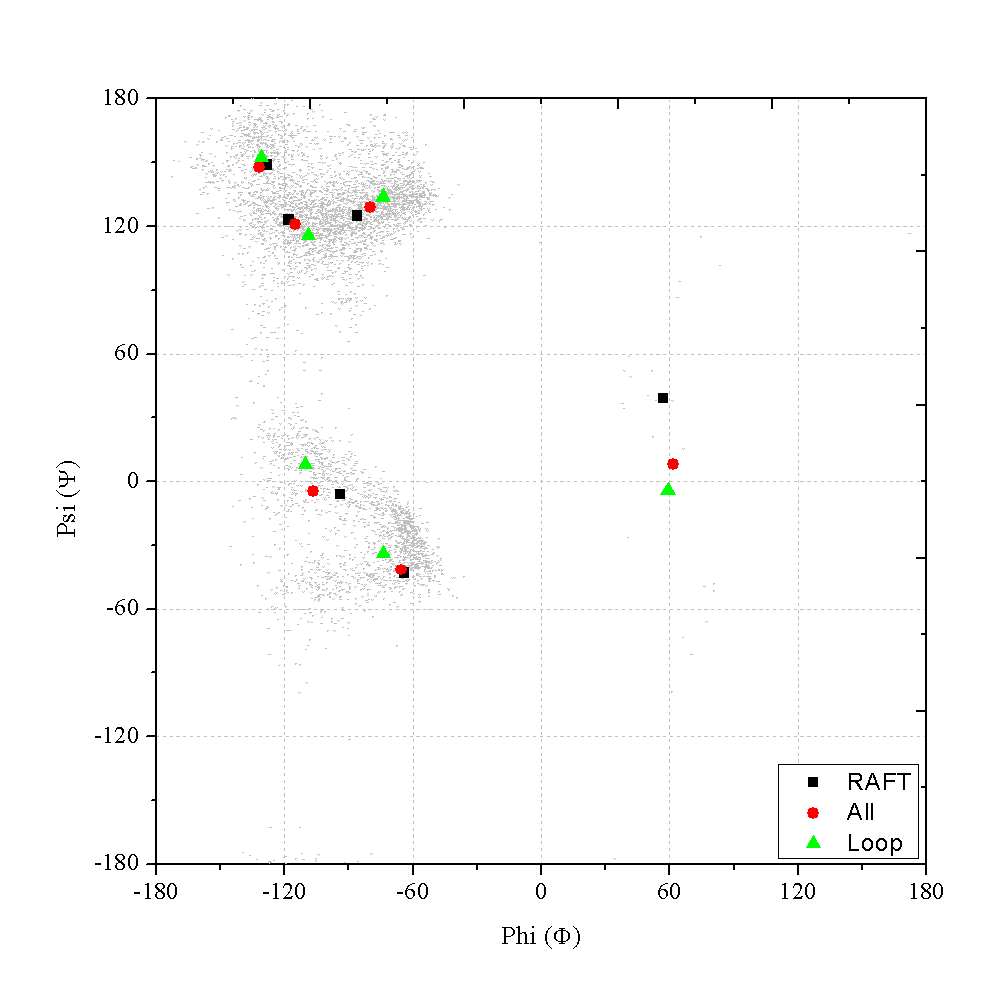
\includegraphics[width=1.0\textwidth]{05-ReducedRep/isoleucine/I_6_0_B_fitgraph.png}}}
      }
    \mbox{
      \subfigure[7 angle allocations]{\scalebox{\anglesetscale}%
      {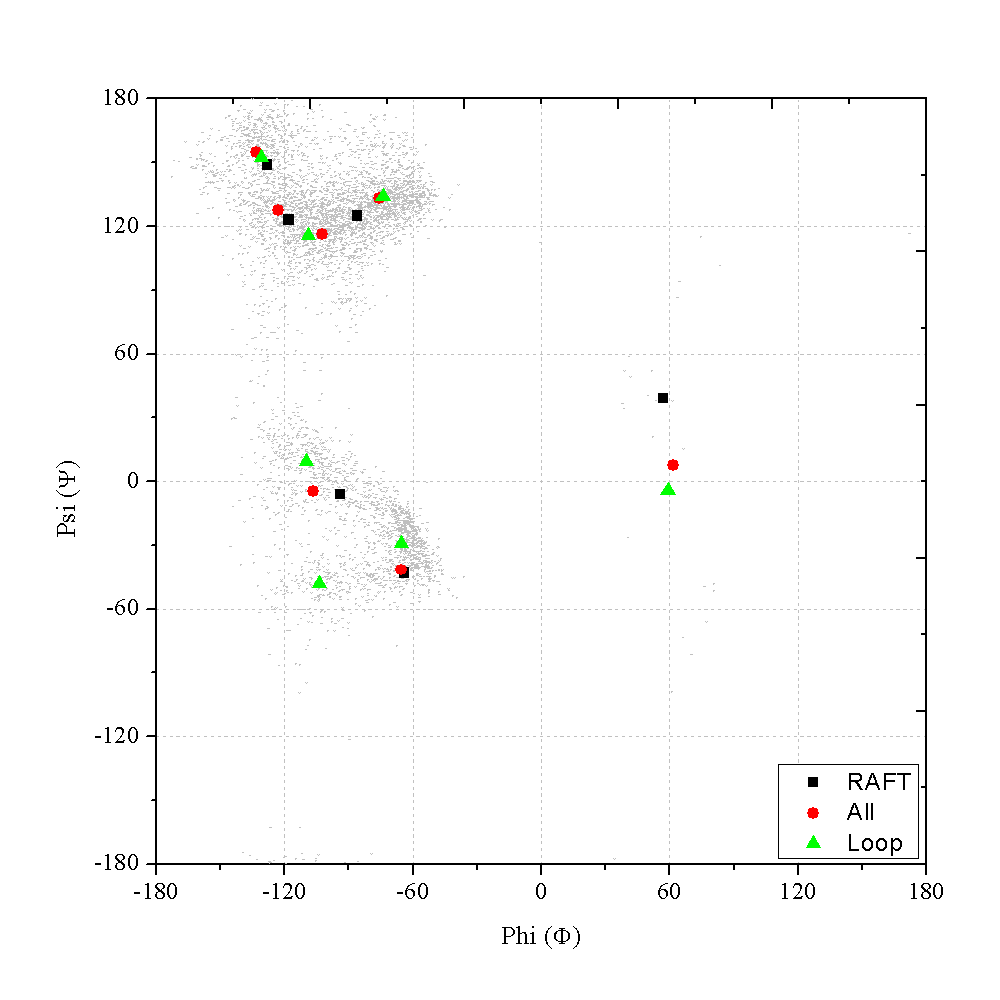
\includegraphics[width=1.0\textwidth]{05-ReducedRep/isoleucine/I_7_0_B_fitgraph.png}}} \quad
      \subfigure[8 angle allocations]{\scalebox{\anglesetscale}%
      {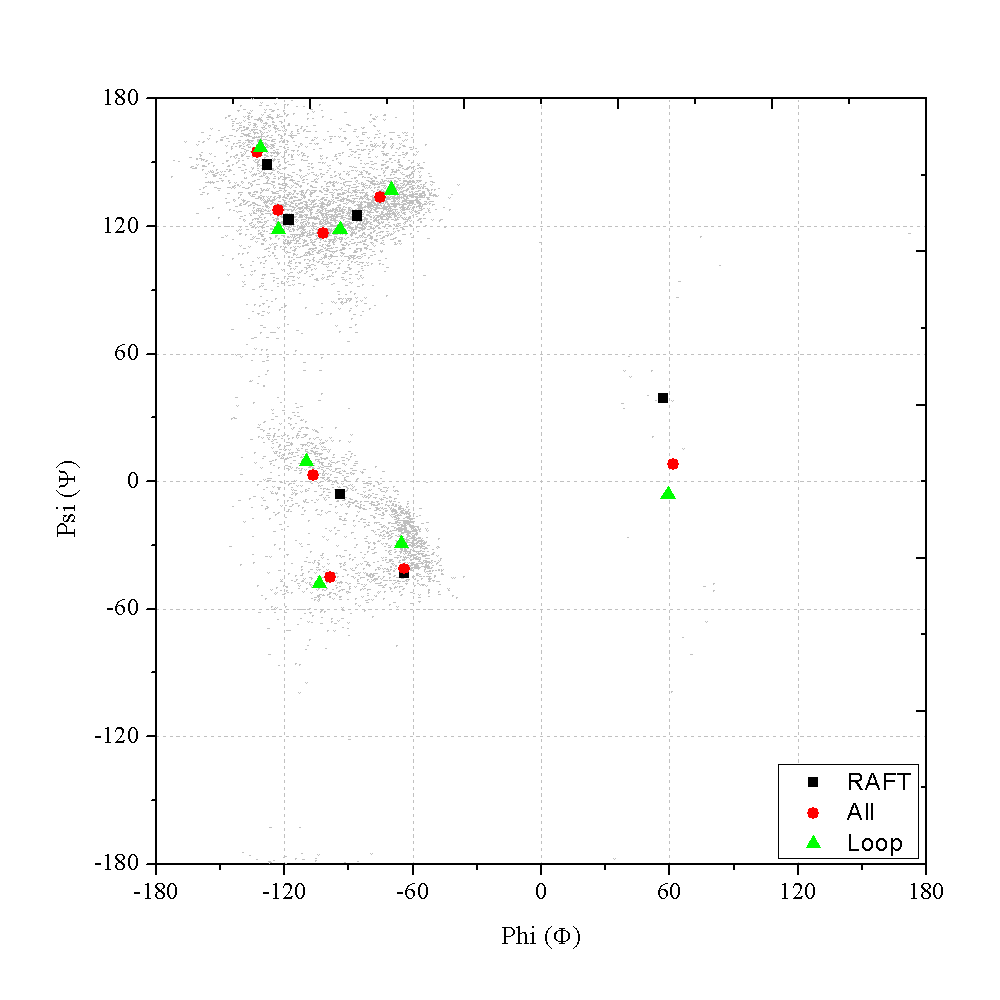
\includegraphics[width=1.0\textwidth]{05-ReducedRep/isoleucine/I_8_0_B_fitgraph.png}}}       }
    \mbox{
      \subfigure[9 angle allocations]{\scalebox{\anglesetscale}%
      {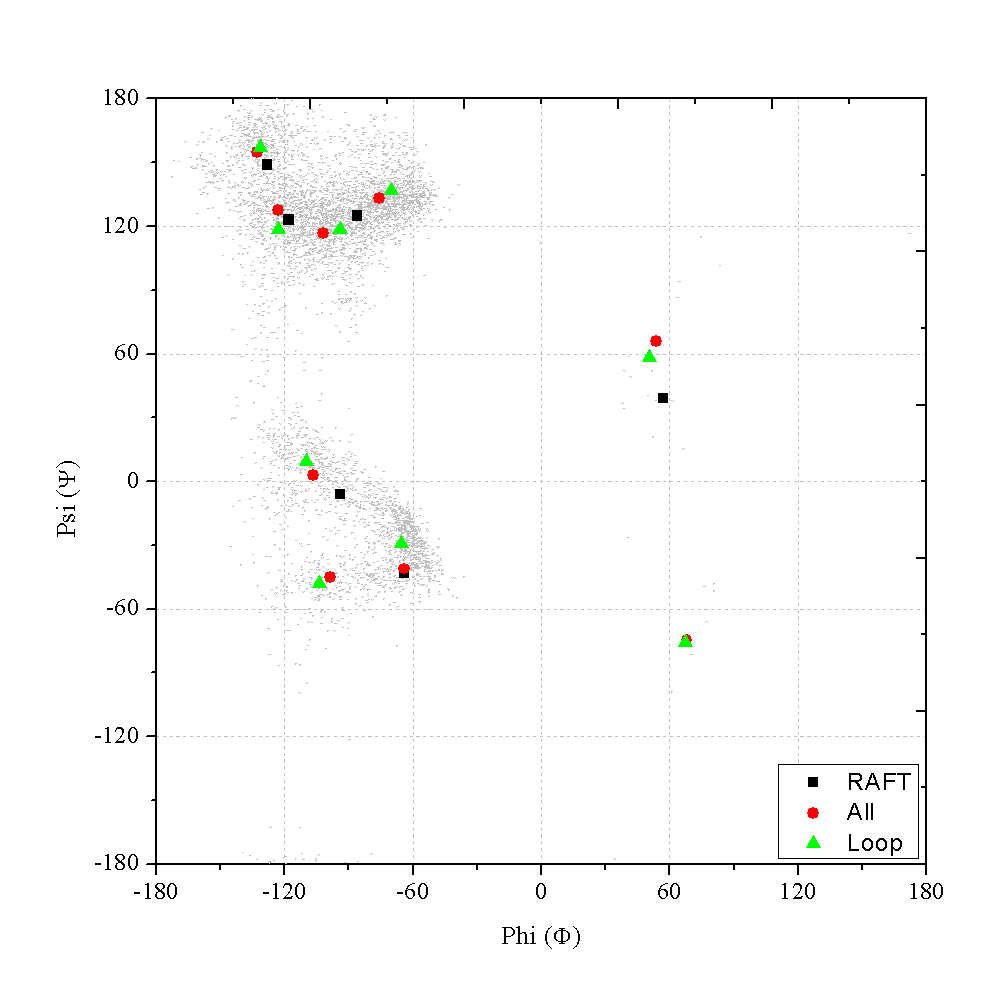
\includegraphics[width=1.0\textwidth]{05-ReducedRep/isoleucine/I_9_0_B_fitgraph.png}}} \quad
      \subfigure[10 angle allocations]{\scalebox{\anglesetscale}%
      {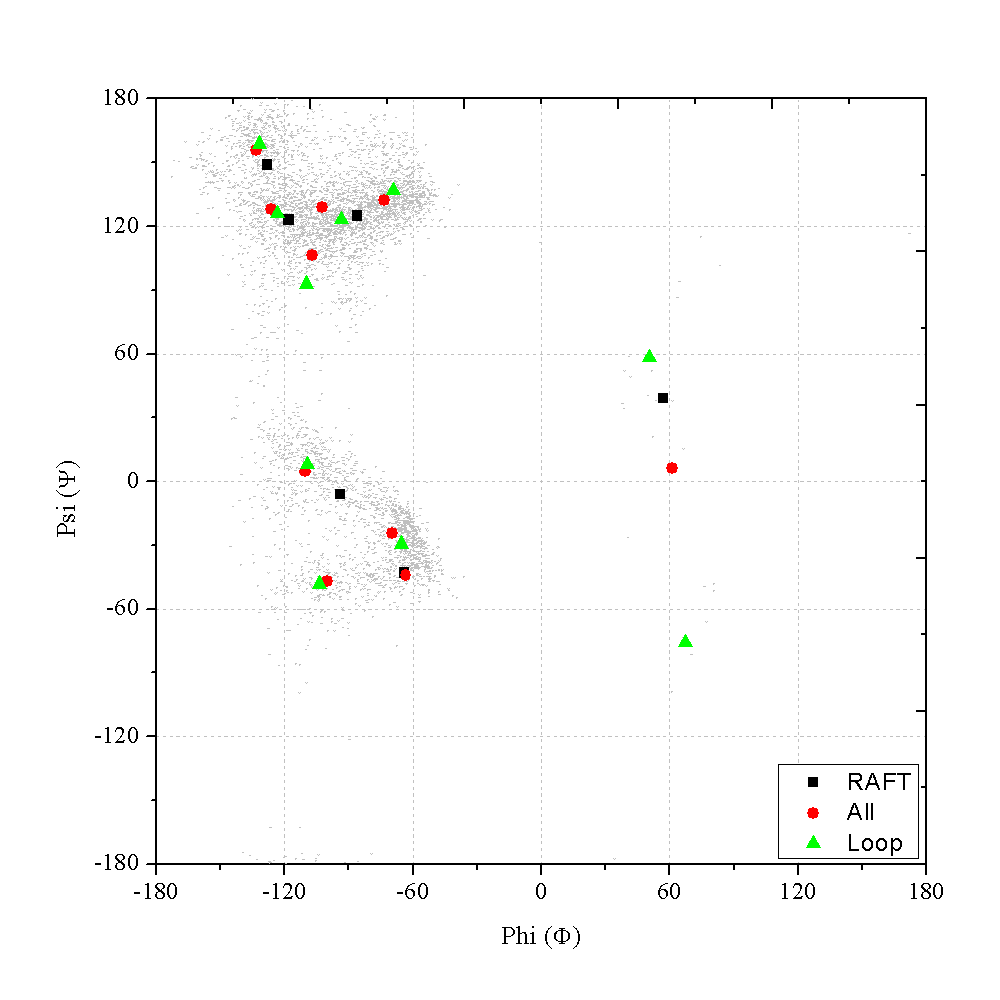
\includegraphics[width=1.0\textwidth]{05-ReducedRep/isoleucine/I_10_0_B_fitgraph.png}}}       }
\caption[Ramachanran distribution and angle fitting for isoleucine]%
{Ramachandran distribution and angle fitting for isoleucine.
Data: 5,395 occurrences (3.33\%) in loop regions only.}
    \label{fig:reducedrep:ramachandran:ile}
  \end{center}
\end{figure}



\subsection{Asparagine: An Extended Beta-region Distribution}

Asparagine stands out as one of the most distinctively-distributed amino acids after glycine and proline. Figure \ref{fig:reducedrep:ramachandran:asn}-a shows a \be-region which is particularity large and sparse where, in contrast to many of the other amino acids, the lower lobes are populated to a greater extent than the centre. Figure \ref{fig:reducedrep:ramachandran:asn}-a also shows that the heft-handed helical region is densely populated for this residue. Figure \ref{fig:reducedrep:ramachandran:asn}-b shows that \be-region fitting is almost identical to that of the original \raft\ study. When adding a \xth{7} angle in figure \ref{fig:reducedrep:ramachandran:asn}-c, there is a difference in fitting-priority between the all-residue and loop-only data-sets. The sparse \be-region is chosen in the all-structure set, whereas the loop-only fitting again chooses to place an angle in disallowed region II. The decision is again reversed when an \xth{8} angle is added in figure \ref{fig:reducedrep:ramachandran:asn}-d.

\begin{figure}[htbp]
  \begin{center}
    \mbox{
      \subfigure[Ramachandran distribution]{\scalebox{\anglesetscale}%
      {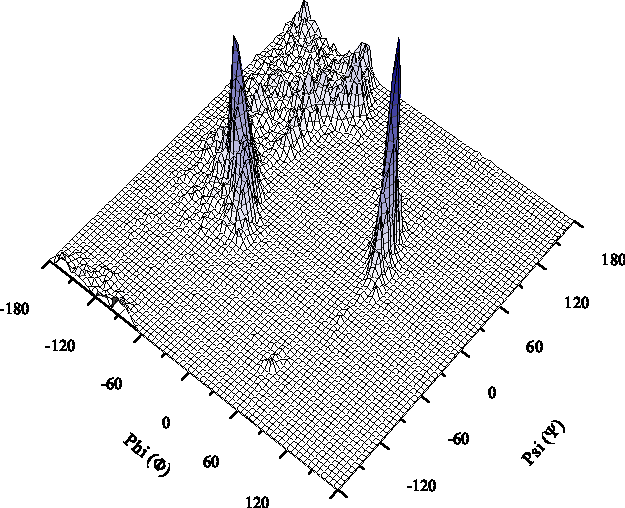
\includegraphics[width=1.0\textwidth]{05-ReducedRep/asparagine/NT_Loop_B_Contour3D.pdf}}} \quad
      \subfigure[6 angle allocations]{\scalebox{\anglesetscale}%
      {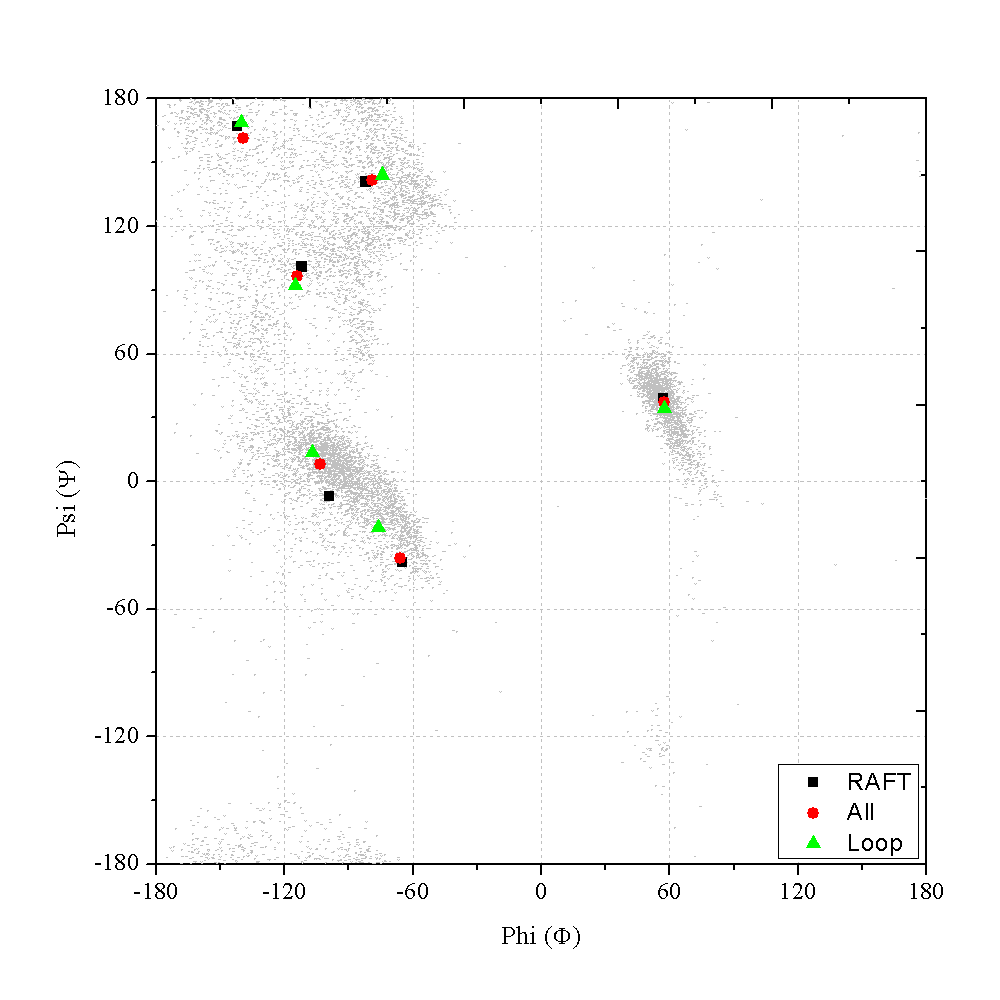
\includegraphics[width=1.0\textwidth]{05-ReducedRep/asparagine/N_6_0_B_fitgraph.png}}}
      }
    \mbox{
      \subfigure[7 angle allocations]{\scalebox{\anglesetscale}%
      {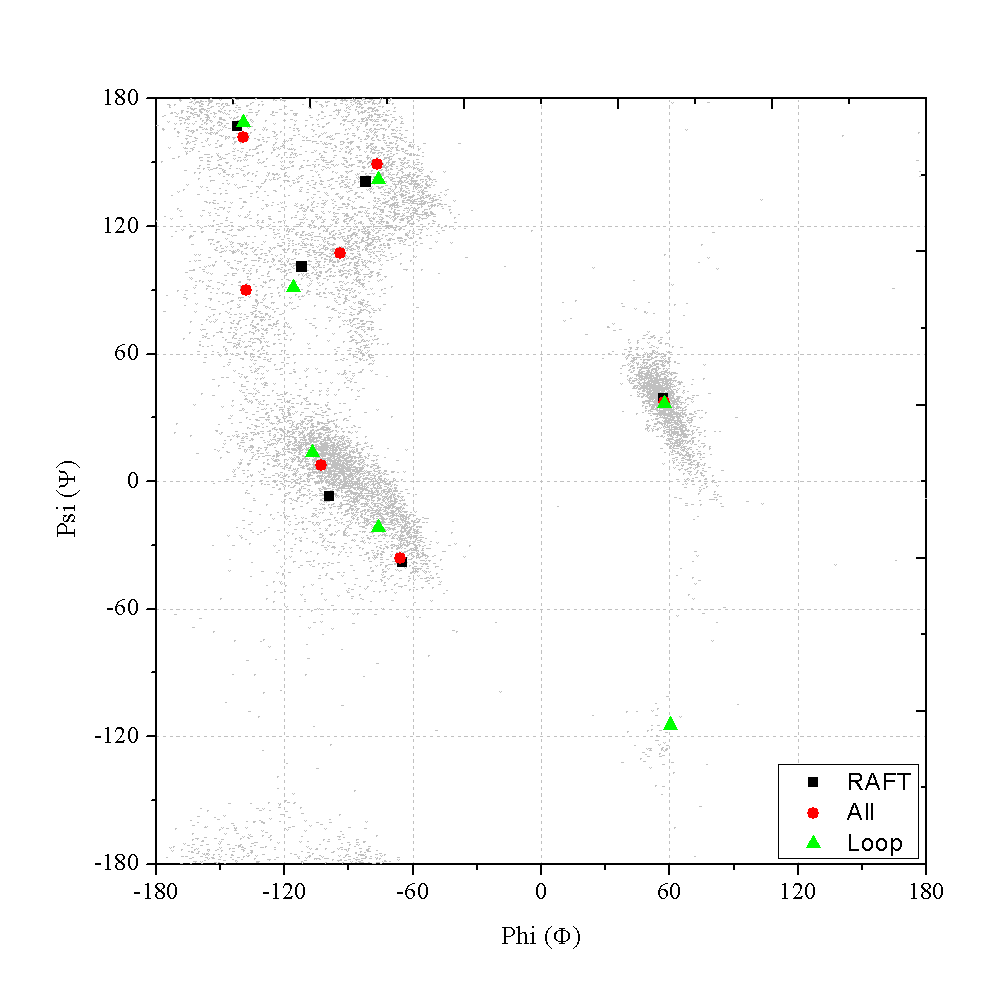
\includegraphics[width=1.0\textwidth]{05-ReducedRep/asparagine/N_7_0_B_fitgraph.png}}} \quad
      \subfigure[8 angle allocations]{\scalebox{\anglesetscale}%
      {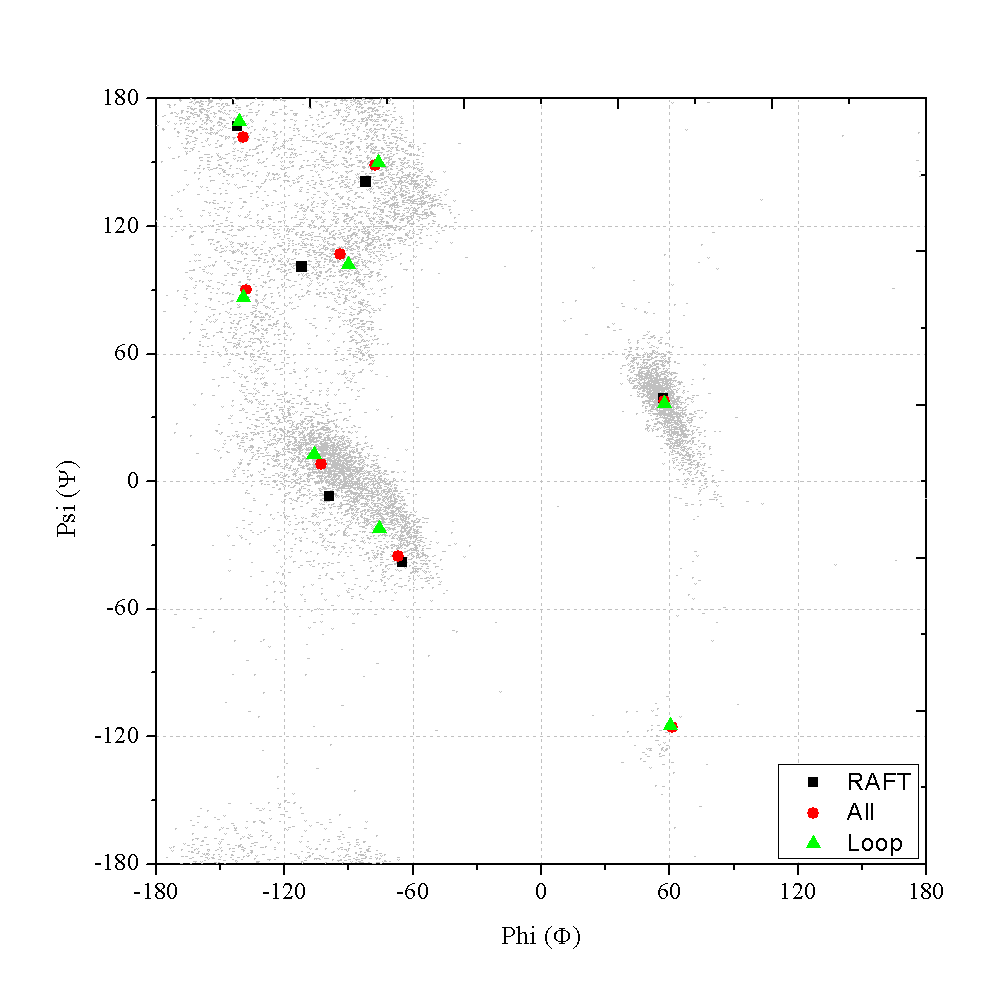
\includegraphics[width=1.0\textwidth]{05-ReducedRep/asparagine/N_8_0_B_fitgraph.png}}}       }
    \mbox{
      \subfigure[9 angle allocations]{\scalebox{\anglesetscale}%
      {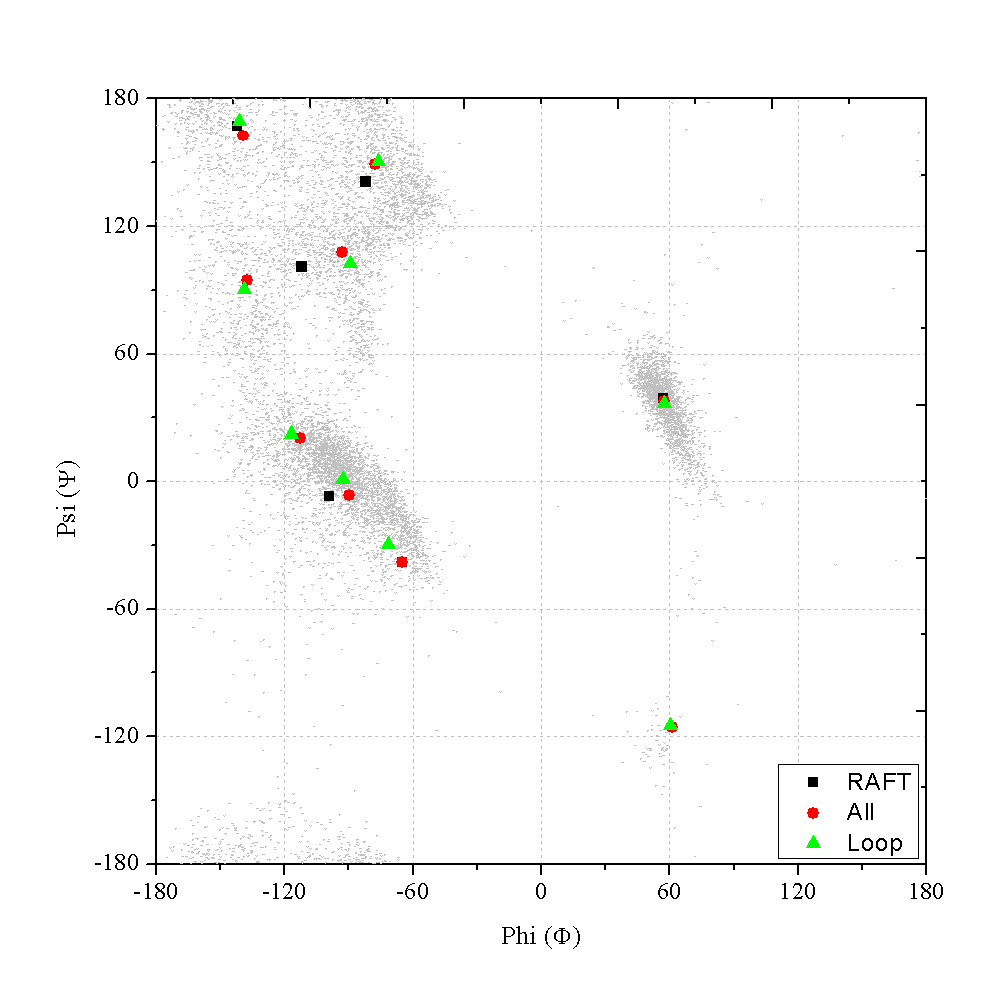
\includegraphics[width=1.0\textwidth]{05-ReducedRep/asparagine/N_9_0_B_fitgraph.png}}} \quad
      \subfigure[10 angle allocations]{\scalebox\anglesetscale
      {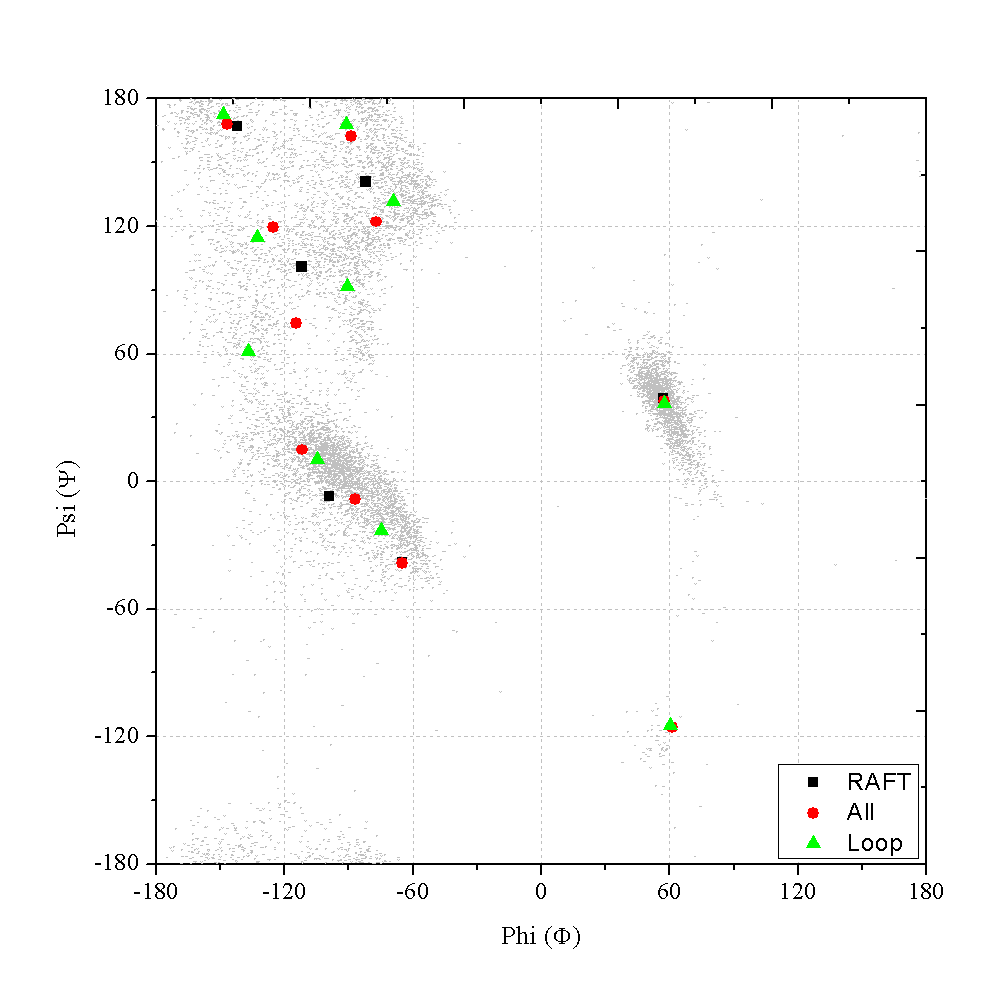
\includegraphics[width=1.0\textwidth]{05-ReducedRep/asparagine/N_10_0_B_fitgraph.png}}}       }
\caption[Ramachanran distribution and angle fitting for asparagine]%
{Ramachandran distribution and angle fitting for asparagine.
Data: 9,802 occurrences (6.04\%) in loop regions only.}
    \label{fig:reducedrep:ramachandran:asn}
  \end{center}
\end{figure}






\subsection{Serine: A Special Case}

As previously discussed, serine is the residue with the most pronounced tendency to occupy disallowed regions, mainly due to the stabilising effect of the hydrogen bonding interactions made by its short polar \sidechain. Other than this, the distribution shown for serine in figure \ref{fig:reducedrep:ramachandran:ser}-a is much like lysine. The most interesting occurrence is shown in 
\ref{fig:reducedrep:ramachandran:ser}-b, where in the fit to the loop-only \dataset, instead of representing the \be-region with the normal three angles, an angle is sacrificed to occupy disallowed region II. The \be-angle is restored in figure \ref{fig:reducedrep:ramachandran:ser}-c when a \xth{7} is added. In addition to this, the all-residue data set also chooses to put the \xth{7} angle in disallowed region II. This second tendency is also shown for other  polar residues D, K and Q, showing that these residue-types must also be above the required density in this region to warrant a fitted angle-pair.



\begin{figure}[htbp]
  \begin{center}
    \mbox{
      \subfigure[Ramachandran distribution]{\scalebox{\anglesetscale}%
      {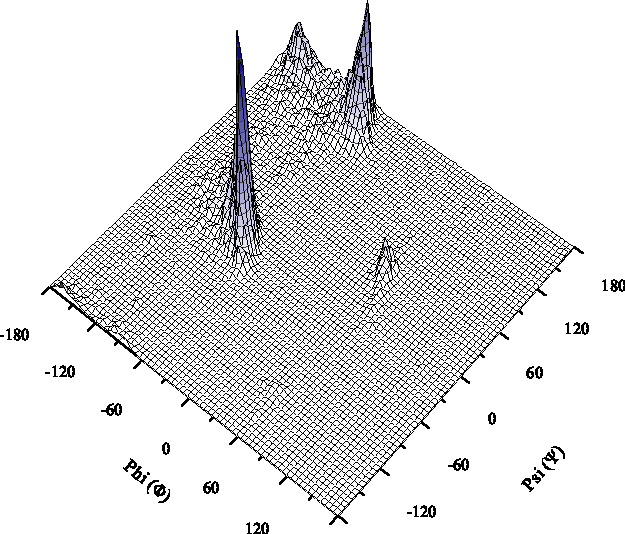
\includegraphics[width=1.0\textwidth]{05-ReducedRep/serine/ST_Loop_B_Contour3D.pdf}}} \quad
      \subfigure[6 angle allocations]{\scalebox{\anglesetscale}%
      {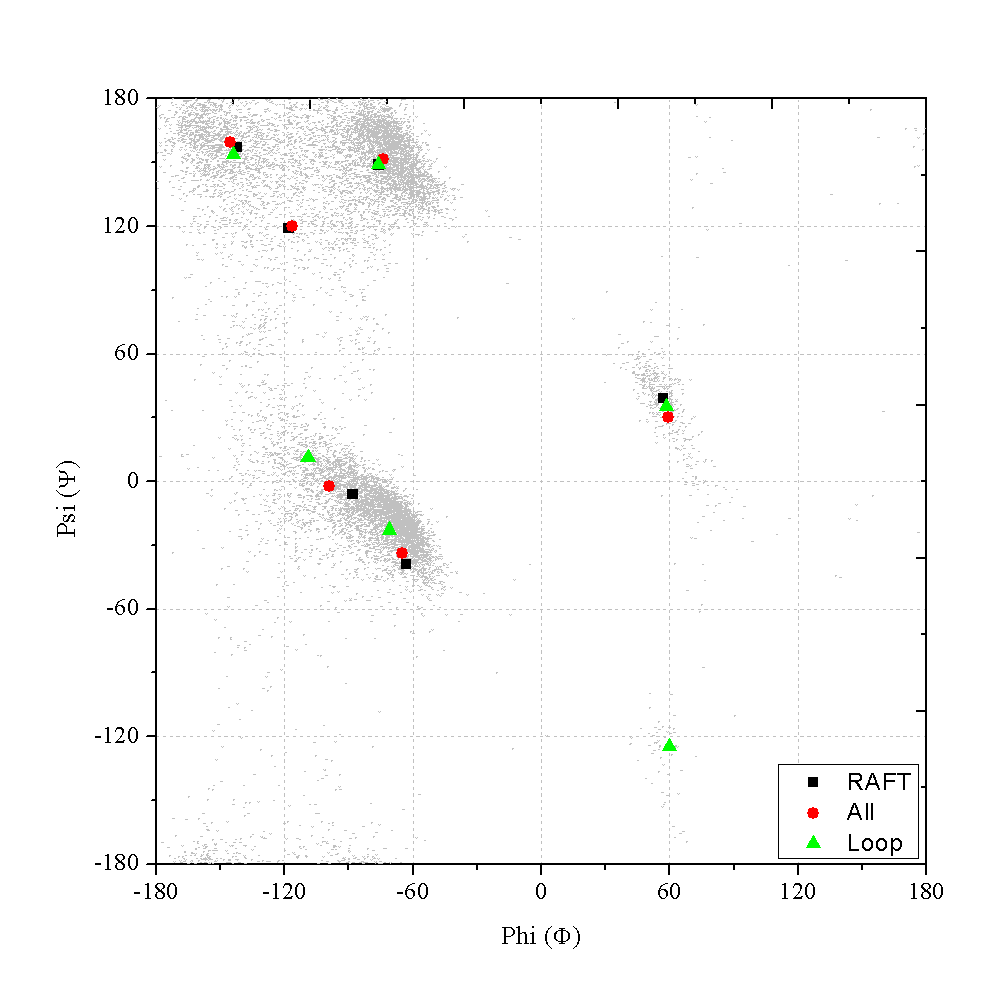
\includegraphics[width=1.0\textwidth]{05-ReducedRep/serine/S_6_0_B_fitgraph.png}}}
      }
    \mbox{
      \subfigure[7 angle allocations]{\scalebox{\anglesetscale}%
      {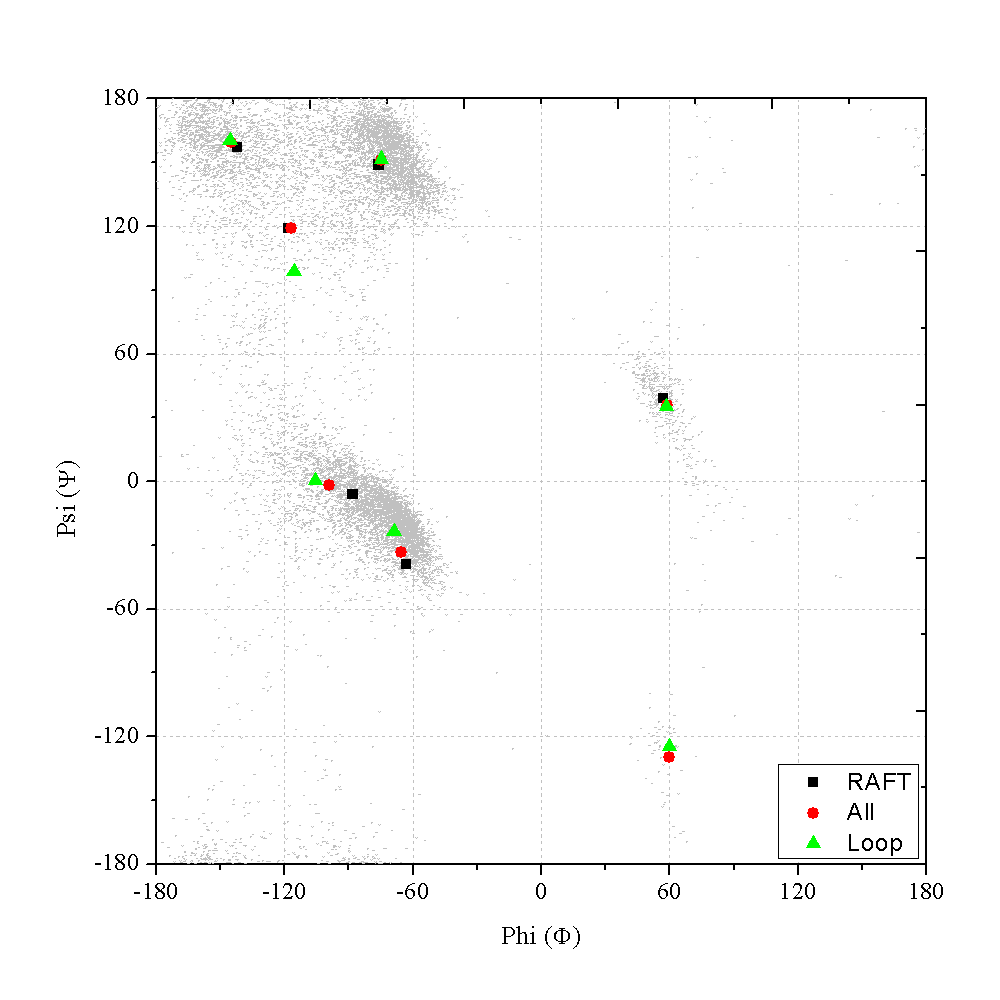
\includegraphics[width=1.0\textwidth]{05-ReducedRep/serine/S_7_0_B_fitgraph.png}}} \quad
      \subfigure[8 angle allocations]{\scalebox{\anglesetscale}%
      {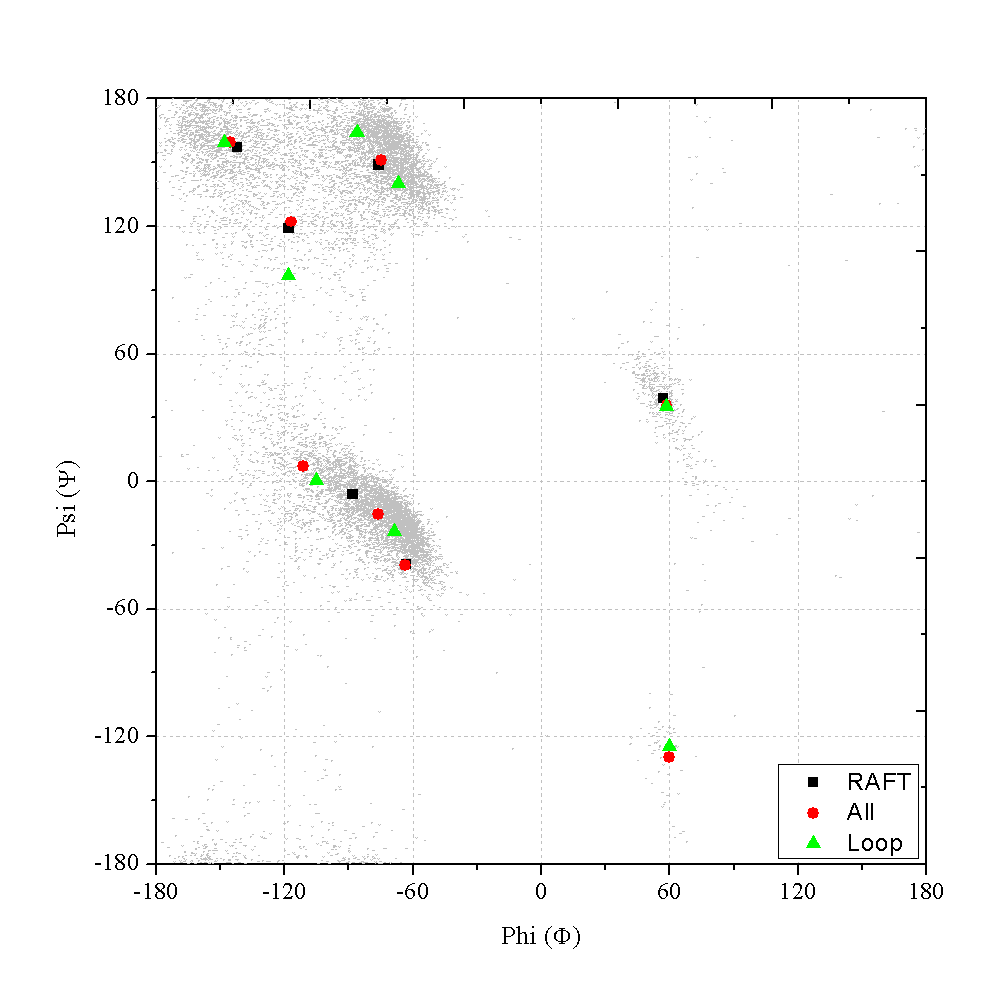
\includegraphics[width=1.0\textwidth]{05-ReducedRep/serine/S_8_0_B_fitgraph.png}}}       }
    \mbox{
      \subfigure[9 angle allocations]{\scalebox{\anglesetscale}%
      {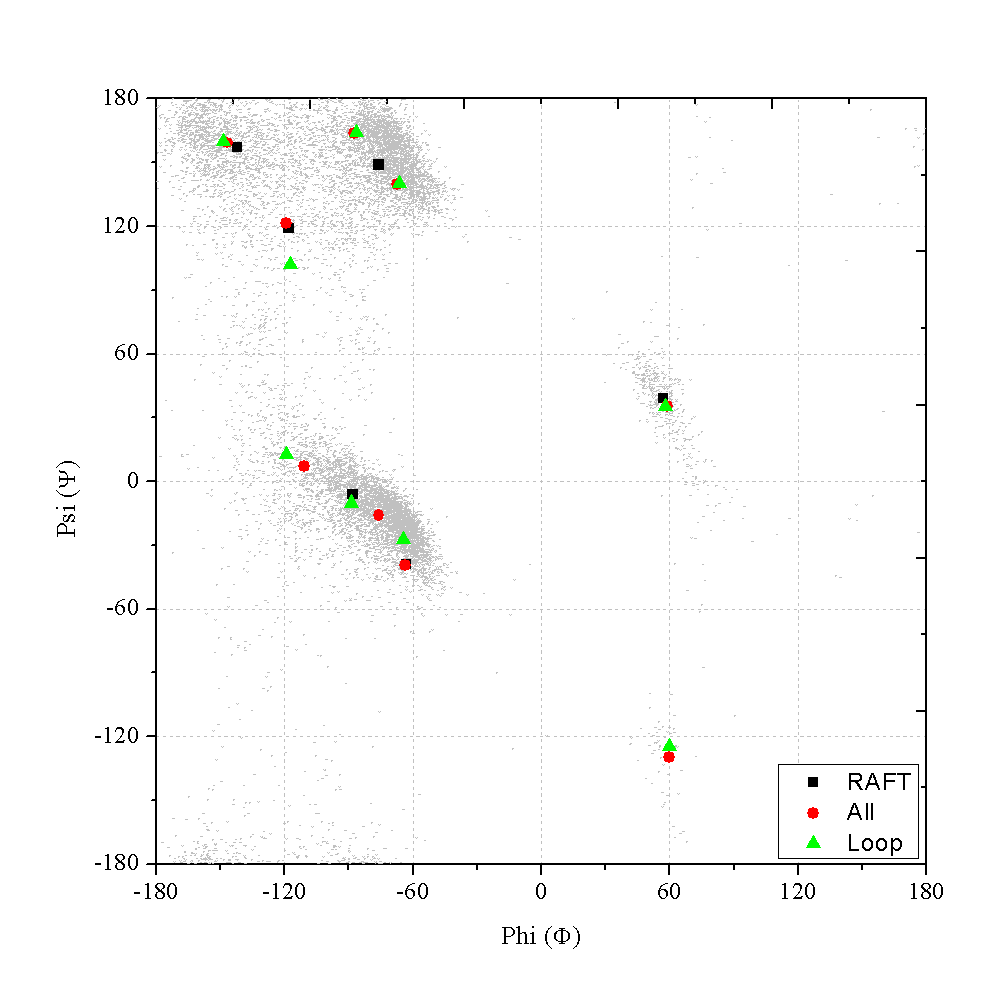
\includegraphics[width=1.0\textwidth]{05-ReducedRep/serine/S_9_0_B_fitgraph.png}}} \quad
      \subfigure[10 angle allocations]{\scalebox{\anglesetscale}%
      {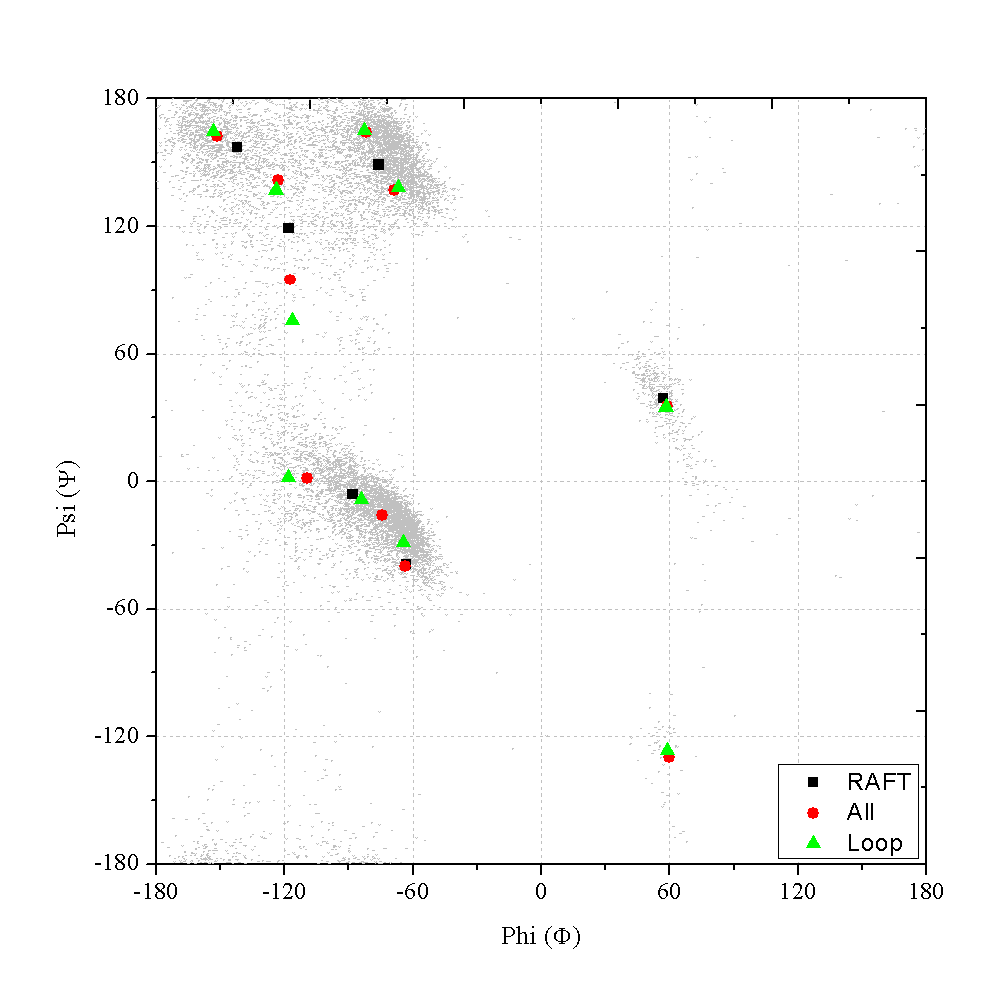
\includegraphics[width=1.0\textwidth]{05-ReducedRep/serine/S_10_0_B_fitgraph.png}}}       }
\caption[Ramachanran distribution and angle fitting for serine]%
{Ramachandran distribution and angle fitting for serine.
Data: 12,164 occurrences (7.50\%) in loop regions only.}
    \label{fig:reducedrep:ramachandran:ser}
  \end{center}
\end{figure}




\subsection{Glycine: A Special Case}

Figure \ref{fig:reducedrep:ramachandran:gly}-a demonstrates that, when compared to the other residues, the Ramachandran distribution for glycine shows fundamental differences. If the circular nature of the plot is taken into account, four distinct regions of population can be seen. The normal \al-region and left-handed helical regions are still present, with a distinct shift in propensity to the latter, which is obviously of great importance in loop regions where glycine is more common. The \be-region density can be seen to have extended upwards to the $\Psi$=-165 region. Both the lower \be-region and the two lower lobe-regions are largely unpopulated. 

Figure \ref{fig:reducedrep:ramachandran:gly}-b shows that glycine represents the greatest deviation between the original \raft\ study and the newer automated fitting procedure. The original study fitted a single angle to the \al\ and left-handed helical regions for glycine in contrast to two angles that were used in the \al-region for all other residue-types. When automated fitting was performed using data from all-structural types, the second \al-helical angle is restored at the expense of $\Phi=$ 90, $\Psi=$ 170. When the automated fitting procedure is applied to the loop-only data, it interestingly produces almost the same result as for the original \raft\ fit. Figure \ref{fig:reducedrep:ramachandran:gly}-c, shows that, as the left-handed helical region occurs vastly more frequently in loop structure, it is given a second angle when fitted for loops-only. 
It is probably true that to properly represent the diffuse data distribution, glycine as an individual case should be given up to nine angles: two \al-region, two left-handed helical, four for the main regions of population around the $\Psi$ = 180 line and one final angle to represent the data spread around the $\Phi$ = 180, $\Psi$ = 180 corner.

\begin{figure}[hbtp]
  \begin{center}
    \mbox{
      \subfigure[Ramachandran distribution]{\scalebox{\anglesetscale}%
      {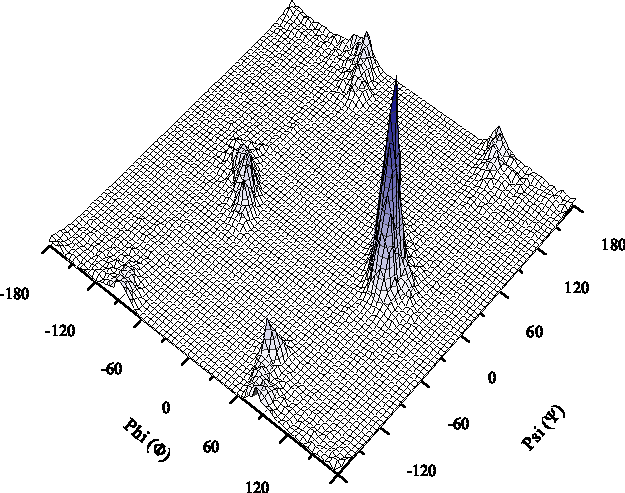
\includegraphics[width=1.0\textwidth]{05-ReducedRep/glycine/GT_Loop_B_Contour3D.pdf}}} \quad
      \subfigure[6 angle allocations]{\scalebox{\anglesetscale}%
      {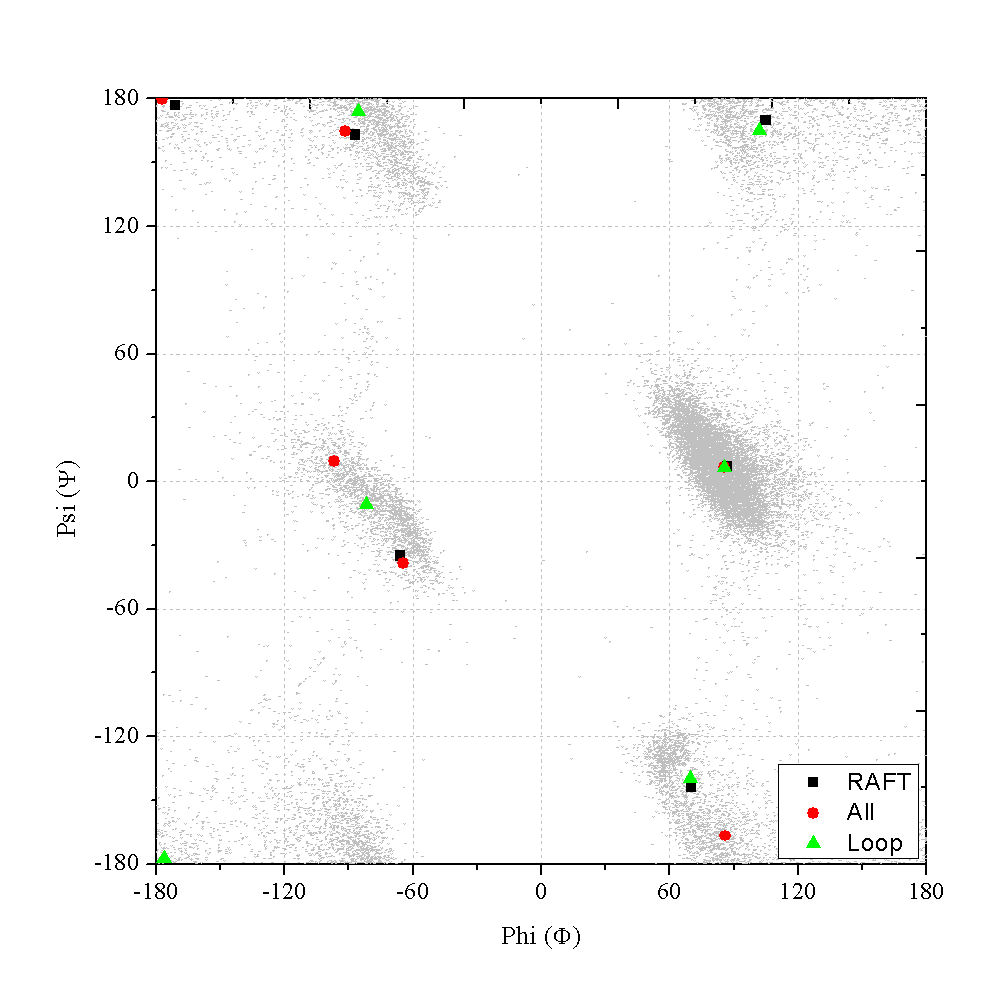
\includegraphics[width=1.0\textwidth]{05-ReducedRep/glycine/G_6_0_B_fitgraph.png}}}
      }
    \mbox{
      \subfigure[7 angle allocations]{\scalebox{\anglesetscale}%
      {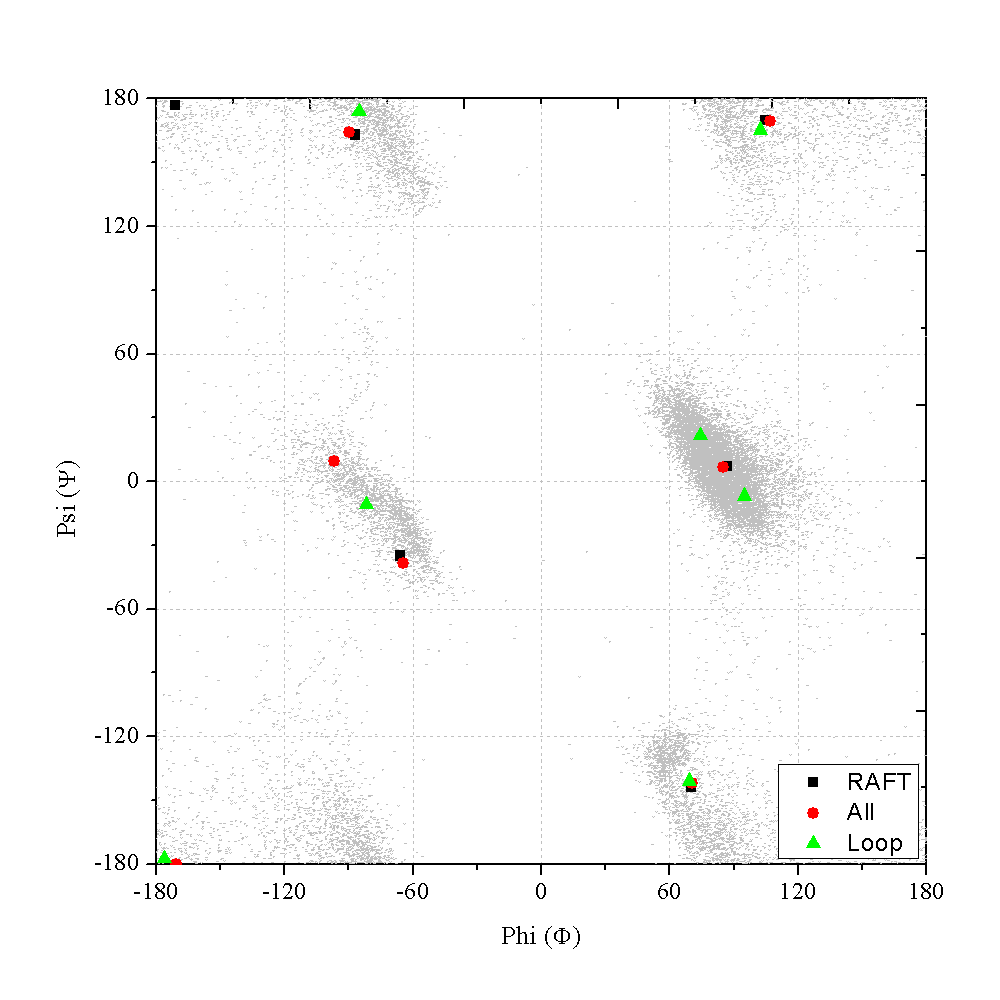
\includegraphics[width=1.0\textwidth]{05-ReducedRep/glycine/G_7_0_B_fitgraph.png}}} \quad
      \subfigure[8 angle allocations]{\scalebox{\anglesetscale}%
      {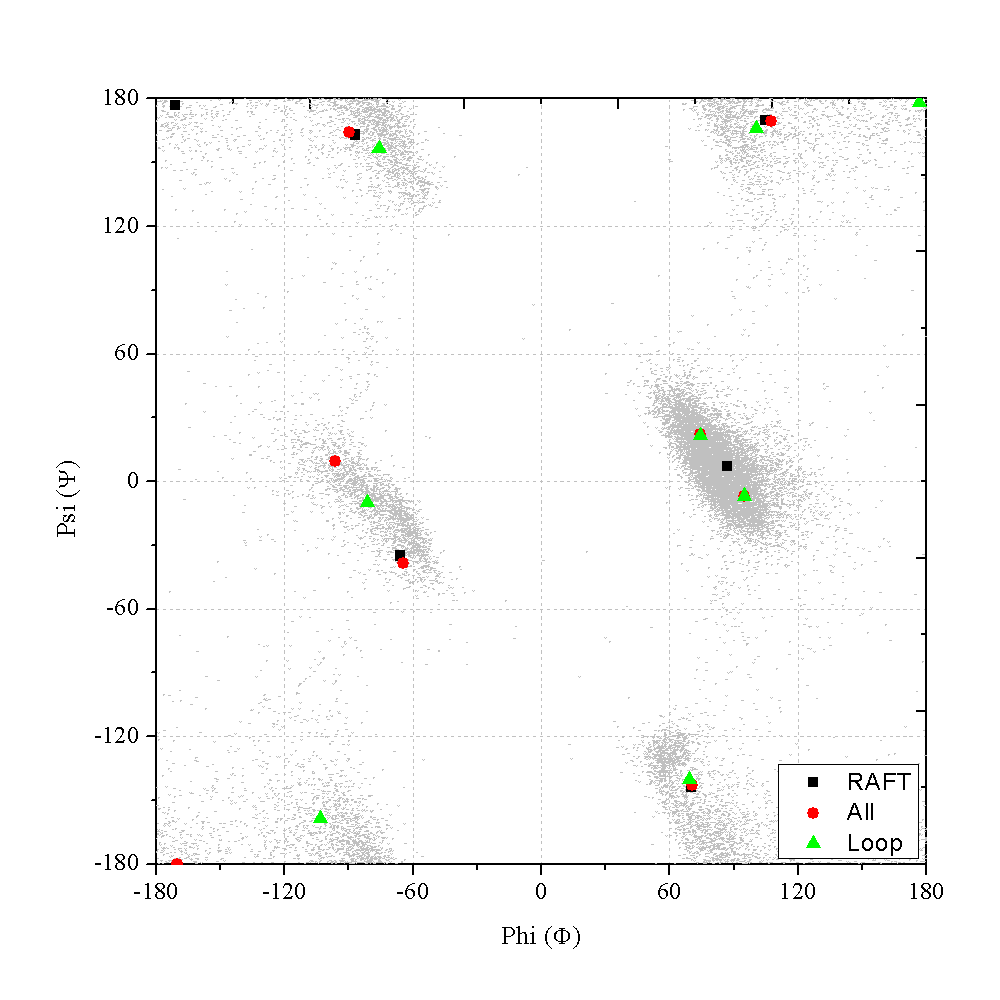
\includegraphics[width=1.0\textwidth]{05-ReducedRep/glycine/G_8_0_B_fitgraph.png}}}       }
    \mbox{
      \subfigure[9 angle allocations]{\scalebox{\anglesetscale}%
      {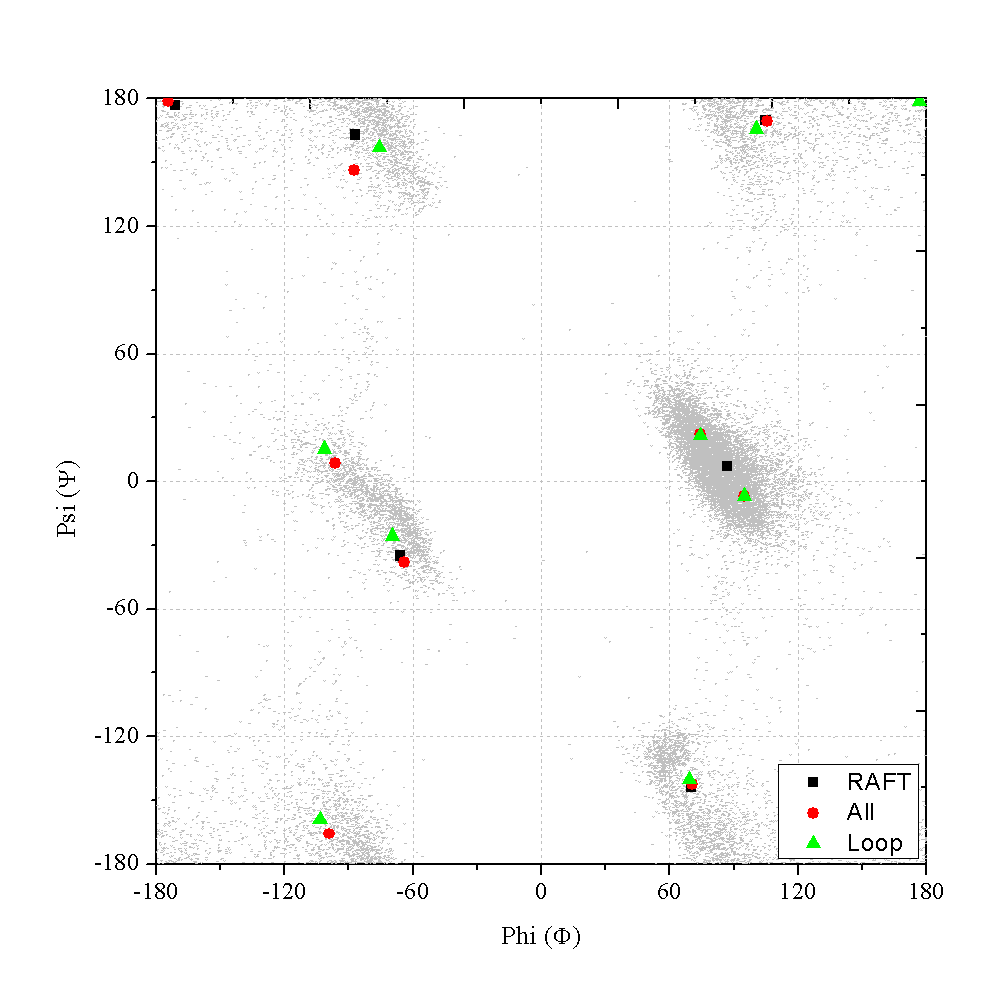
\includegraphics[width=1.0\textwidth]{05-ReducedRep/glycine/G_9_0_B_fitgraph.png}}} \quad
      \subfigure[10 angle allocations]{\scalebox{\anglesetscale}%
      {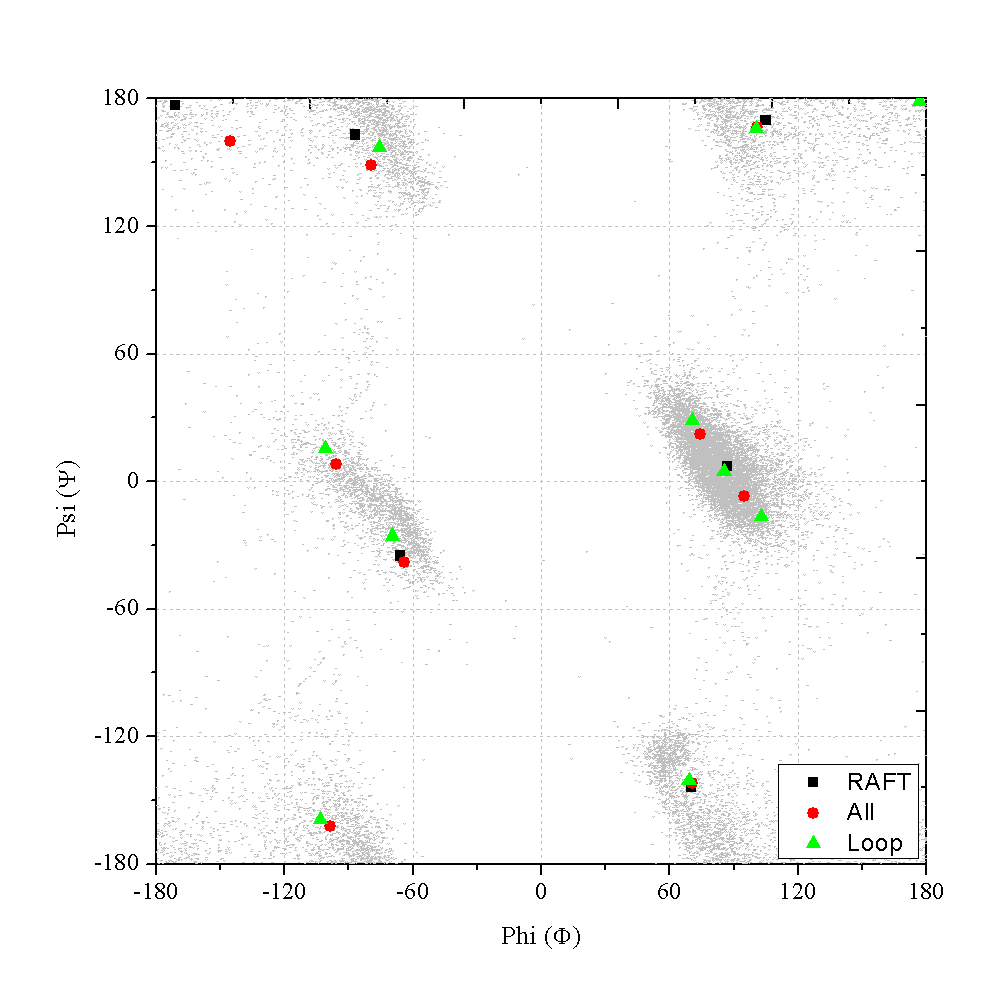
\includegraphics[width=1.0\textwidth]{05-ReducedRep/glycine/G_10_0_B_fitgraph.png}}}       }
\caption[Ramachanran distribution and angle fitting for glycine]%
{Ramachandran distribution and angle fitting for glycine.
Data: 20,021 occurrences (12.34\%) in loop regions only.}
    \label{fig:reducedrep:ramachandran:gly}
  \end{center}
\end{figure}


% -----------------------------------------------------
% Proline-specific as the caption is larger, 
% withough causing float overflow...
\renewcommand{\anglesetscale}{0.408}
% -----------------------------------------------------

\subsection{Proline: A Special Case}

Finally, figure \ref{fig:reducedrep:ramachandran:pro}-a illustrates the constrained nature of the $\Phi$ torsion in proline; the overall distribution being clearly more limited than for other residues. By comparing the plots, it can be seen that the distribution for cis-proline is shifted slightly in the negative-$\Phi$ direction. 

The majority of data lies in two peaks centred around $\Psi$=140 and $\Psi$=40, however there is a lightly populated central region centred around $\Psi$=60, but only for the trans-form. This reveals a slight oversight during fitting in the original \raft\ study, due to the use of  pre-defined human-selected regions, where the \third\ populated region for proline was not considered. Figure \ref{fig:reducedrep:proreg3} shows a well resolved example of this angle-pair from \thothdb. 

From the plots it can be seen that four and three angle-pairs for trans and cis-proline respectively are most likely a waste of additional complexity, as two fitted angle-pairs both reside within a tight, circular distribution. This sharing may actually be detrimental to the stage 2 search process as more unpopulated space will be included within the circular search radii. From these considerations, it was decided that the best representation for proline, no matter how many angle allocations were given to other residues, should be three angle-pairs for trans-proline and two angle-pairs for cis-proline.



\begin{figure}[htbp]
  \begin{center}
    \mbox{
      \subfigure[Trans Ramachandran distribution]{\scalebox{\anglesetscale}%
      {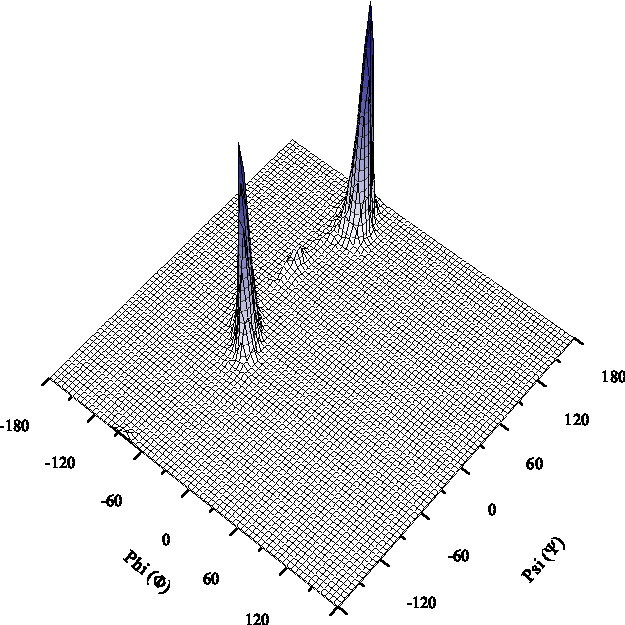
\includegraphics[width=1.0\textwidth]{05-ReducedRep/proline/PT_Loop_B_Contour3D.pdf}}} \quad
      \subfigure[Cis Ramachandran distribution]{\scalebox{\anglesetscale}%
      {\includegraphics[width=1.0\textwidth]{05-ReducedRep/proline/PC_Loop_B_Contour3D.pdf}}}
      }
      \vspace{0.5cm}
    \mbox{
      \subfigure[Trans proline\superscript{a}: 3 angle allocations]{\scalebox{\anglesetscale}%
      {\includegraphics[width=1.0\textwidth]{05-ReducedRep/proline/pT_3_0_B_fitgraph.png}}} \quad
      \subfigure[Cis proline\superscript{b}: 2 angle allocations]{\scalebox{\anglesetscale}%
      {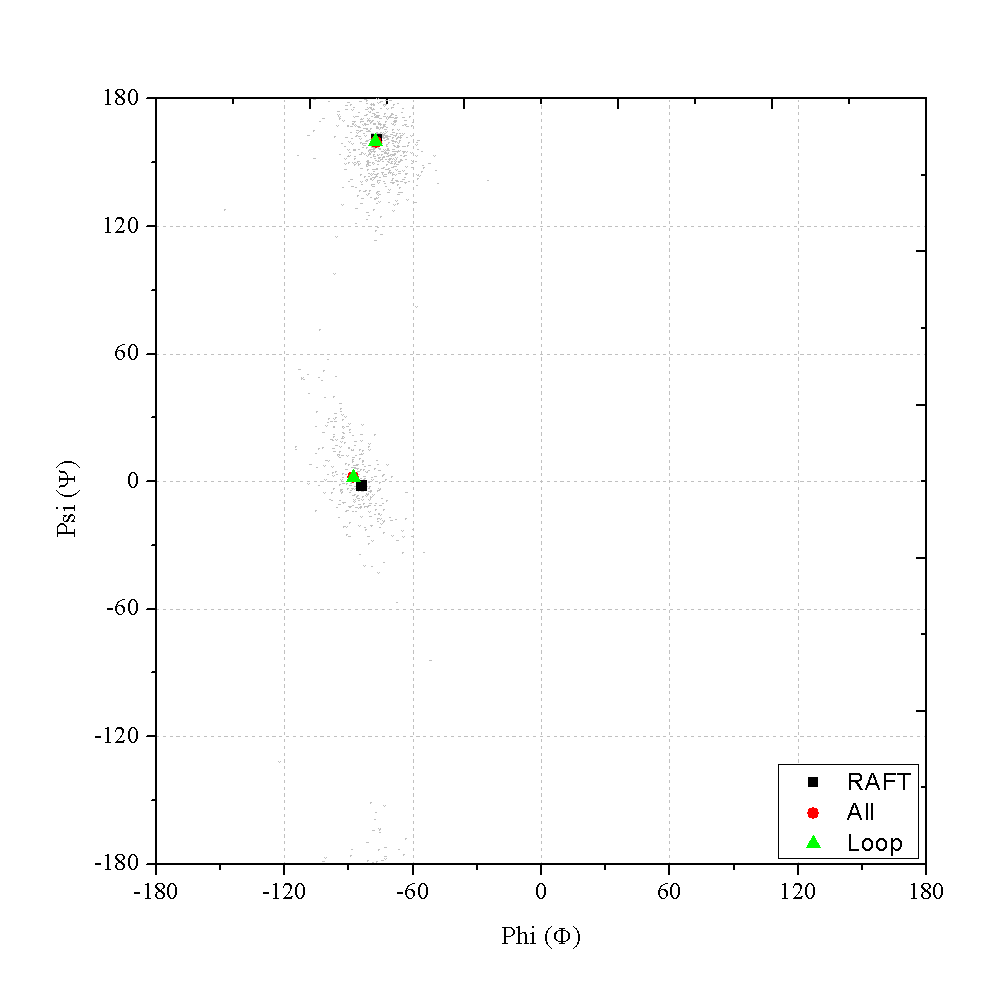
\includegraphics[width=1.0\textwidth]{05-ReducedRep/proline/pC_2_0_B_fitgraph.png}}}       }
      \vspace{0.5cm}
    \mbox{
      \subfigure[Trans proline\superscript{a}: 4 angle allocations]{\scalebox{\anglesetscale}%
      {\includegraphics[width=1.0\textwidth]{05-ReducedRep/proline/pT_4_0_B_fitgraph.png}}} \quad
      \subfigure[Cis proline\superscript{b}: 3 angle allocations]{\scalebox{\anglesetscale}%
      {\includegraphics[width=1.0\textwidth]{05-ReducedRep/proline/pC_3_0_B_fitgraph.png}}}       }
\caption[Ramachanran distribution and angle fitting for proline]%
{Ramachandran distribution and angle fitting for cis and trans proline.
Data\superscript{a}: 11,179 trans occurrences (6.89\%) in loop regions only. Data\superscript{b}: 887 cis occurrences (0.55\%) in loop regions only.}
    \label{fig:reducedrep:ramachandran:pro}
  \end{center}
\end{figure}


\begin{figure}[hptb]
\begin{center}
\includegraphics[width=0.7\textwidth]{05-ReducedRep/pro_reg3/pro_reg3.png}
\caption[Structural illustration of a third populated region of the Ramachandran plot]{Structural illustration of a third populated region of the Ramachandran plot: The structural data shown is a \mer{9} loop in 1R77A from residue 297, containing a proline residue occupying the central low-population
region of the Ramachandran map at $\Phi$=-77.5 and $\Psi$=62.2.  The \ca\ B-factor for Pro-300 is $12.0$\AA$^2$;  of high enough quality
to be included in any structural study.
The proline, loop and anchor residues are shown in yellow, green and magenta
respectively. Image created with \pymolV. }
\label{fig:reducedrep:proreg3}
\end{center}
\end{figure}


\subsection{The Optimised Angle-sets}
\label{section:reduced_rep:optimised_angleset}

Figure \ref{fig:reducedrep:anglesetres} shows a measure of the improvement of the \angleset\ in its ability to represent the data in the database. It can be seen that, as one would expect, an increase in the number of angles yields a greater coverage of available data within a smaller radius around each representative angle. The fitted six-angle set shows a marked improvement over the original \raft\ six-angle set for loop-only structural data. A second interesting observation is that both six-angle sets fit to a double-sigmoid with a small second increase in coverage at around a 140\degree\ influence radius. This is due to the lack of a representative angle to cover the disallowed clusters II and III in these sets. By increasing to a seven \angleset, there is an additional marked improvement in coverage and this minor second phase is no longer present.

\begin{figure}[hptb]
\begin{center}
\includegraphics[width=0.7\textwidth]{05-ReducedRep/closest_angle/IncreaseResolution.pdf}
\caption{Graphical representation of angle coverage of different \anglesets.}
\label{fig:reducedrep:anglesetres}
\end{center}
\end{figure}

As the most marked improvement was obtained simply by re-parametisation of six angle-pairs, and also for best comparison with the original \raft\ work, the primary \angleset\ used throughout this work is still based on the use of six angles. Two exceptions are glycine which is given eight angle-pairs due to its increased conformational variability and proline which is assigned five mixed-cis-trans angle-pairs. This set is termed the optimised 6-8-5 \angleset. A second \angleset\ was also defined which increased the overall resolution by allocating eight angle-pairs to all-residue types, ten to glycine and again five to proline. This set is termed the optimised 8-10-5 \angleset. From figure \ref{fig:reducedrep:anglesetres}, it can be estimated that to obtain over 90\% data coverage, a 60\degree\ maximal search radius is required for the 6-8-5 \angleset\ and a 50\degree\ radius for the 8-10-5 \angleset.
The exact optimised \anglesets,\ with associated probability data, are presented in appendix \ref{appendix:angleset}.

\section{Comparison to Other Published Methods}

Current examples in the literature generally utilise angle-sets that are parametised from the averaged data taken from all structural types, including secondary structures.  If propensity information was to be derived for this data, it would be heavily biased towards the \al-helical states. Some current methods use fine-grained grid-based  \anglesets\ which have no propensity-weighting, but simply mark \phipsi\ states on or off\cite{METHOD:Plop,METHOD:RapperB}. Such parametisations can not be searched exhaustively and rely upon sampling to find valid conformations. Other methods do not rely on discretised values at all, choosing instead, sampling under an empirical potential of mean force (PMF)\cite{METHOD:Modloop} -- these again rely on sampling.
All of these methods are discussed in more detail in chapter \ref{chapter:methods}.

In this work, it was shown that there is a significant difference in propensity between different structural-states when using the all-structure and loop-structure databases. Loop-structure also shows a larger deviation in possible \phipsi\
states, representing the majority of the sparse outlying data on the Ramachandran
plot.
Such information is, therefore, likely to be important and has therefore been derived in combination with the \angleset\ produced in this work. The success of this coarse-grained approach will be assessed and discussed further in the following chapters. 
  

\section{Conformer Building}

As discussed in section \ref{section:complexity}, it is impossible to know from the outset whether or not a given conformer will be a viable loop candidate. Therefore, to find viable candidates, large numbers of possible conformers must be generated and screened for viability. This section outlines this process.


\subsection{The Structural Model and Conformer Selection}

To make the transition from conformer-descriptor to coarse loop-model, the conformer must be attached to the protein body, which can be performed via a multitude of different approaches. One method could be to build and assess loop fragments in isolation and then to stitch selected candidates onto the protein body anchor residues, which is used in the method \petra\cite{METHOD:Petra}. This approach, however, is not computationally efficient for two reasons. Firstly, in order to perform any docking process, additional anchor-residues are required on the protein loop-candidate for use in superimposition onto the complementary rigid-body anchors. This means that the loop candidate is longer than the loop itself and therefore more computationally costly. Secondly, optimal docking of the loop-anchors  onto the anchor-residues is a non-trivial process. Following superimposition, multiple pose assessments would be required to find an optimum which fitted against the other atoms in the protein body. 

A second more viable option is to grow the conformation out of one or both anchors. This side-steps any need for subsequent fragment docking, providing a significant performance gain.  This is the chosen method for this work. During development, it was decided that the simplest and most effective way would be to build the conformer extending away from the N-terminus, using idealised geometry and only the \bbatoms. This is shown diagrammatically in figure \ref{fig:reduced_rep:conformer}-a. Main-chain rotations can then be efficiently performed in the context of the protein body and viable conformer-descriptors stored in a list for subsequent refinement (chapter \ref{chapter:prearcus}).
 
\begin{figure}[hptb]
\begin{center}
\subfigure[Loop definition]{\includegraphics[width=0.45\textwidth]{05-ReducedRep/conformer/loop_definition.pdf}}
\subfigure[Conformer selection logic]{\includegraphics[width=0.45\textwidth]{05-ReducedRep/conformer/logic.pdf}}
\end{center}
\caption{The coarse-resolution conformer model.}
\label{fig:reduced_rep:conformer}
\end{figure}

In order to accommodate a break in the \mainchain, the standard atom-definitions for the $\Psi$- torsion was reassigned from \mbox{N--\ca--C--N$_\text{(n+1)}$}  to be \mbox{N--\ca--C--O}; where \mbox{$(n+1)$} signifies the following residue. This was done because, if the standard definition was used, the $\Phi$-angle of the terminal residue would be measured and transformed using the coordinate of the next residues N-atom.  Due to the bond-break in a coarse model, this atom would almost exclusively be in a nonsensical relative location. As idealised-geometry is used throughout conformer-enumeration, whereby the peptide group is always perfectly planar, this definition change has no effect in real terms. 

Conformer viability is determined by a filtering process, illustrated in figure \ref{fig:reduced_rep:conformer}-b. After a given conformer has been applied, two independent filters are invoked. The first filter is trivial to compute per-conformer, being simply the distance between the C-atom  at the end of the built conformer and the C-terminal anchor's N-atom. For computational efficiency the square of the distance tested against a user-defined squared distance-cutoff with a default value of 2.0\AA. Early versions of the algorithm also compared the angle formed between the unit directional-vectors of the  \ca--C at the end of the loop and the N--\ca\ of the anchor. This test was later found, by visual trajectory assessment, to provide no appreciable benefit and was therefore discarded. Essentially, the test showed no discrimination with regard to which conformers would remain viable after the following refinement   stage.

The second filter was designed to screen conformers which exhibited excessive steric interaction with the protein core. To assess this quickly, without calculating distances between all loop-atoms and all protein-body atoms, a rapid alternative was devised and is illustrated in figure \ref{fig:reduced_rep:surface}.

\begin{figure}[hptb]
\begin{center}
\includegraphics[width=0.75\textwidth]{05-ReducedRep/conformer/surface_cache.pdf}
\end{center}
\caption[The definition for a surface-atom clash-box]{The definition for a surface-atom clash-box.
The approximate maximum-reach of the loop itself is shown as a red-dashed line.
The N and C-terminal anchors are shown, in combination with three orthogonal axes, built around them using the length of the
maximum-reach path. 
All \ca-atoms which fall within this box, which are not part of the loop itself, are deemed surface atoms.
}
\label{fig:reduced_rep:surface}
\end{figure}

The approximate value of a typical sequence-neighbour \ca--\ca\ distance is 3.8\AA. So by multiplying this by the number of residues in the loop, a crude maximum-travel distance is obtained. If one then imagines this distance as a string pulled tight away from the anchor residues, one can obtain distances along three orthogonal coordinates, X', Y' and Z', which define a cuboid containing all atoms that can possibly interact with the loop. As none of the protein-core atoms move during simulation, one can store a list of \ca\ atoms for use in steric checks against the current conformer. Surface-atoms other than \ca-atoms could easily be included, but would greatly increase the cost of calculation.

In figure \ref{fig:reduced_rep:surface}, the Y'-axis is orientated such that it is perpendicular to the C--N vector of the N-terminal anchor. The X'-axis is orientated so that it lies along the path from the N-atom of the C-terminal anchor to the C-atom of the N-terminal anchor, where $d$ is the distance from the origin to each anchor and is equal for both. The red dashed-line shows the maximum-travel distance
extruded to its maximal reach along the Y'-axis; the same can be done for the Z'-axis. By simply solving a right-angle triangle we obtain the size of the box for both the Y' and Z' axes. The reach along the X'-axis is simply $(3.8n - 2d) / 2 + d$, which simplifies to $1.4n$.
Finally, to reduce the number of atoms, the distance along the negative Y'-axis is reduced by an empirical scaling-factor of 75\%. This is because, due to the orientation of the box, if the loop clashes with an atom at the bottom of the box, then it should also have clashed with an atom higher in the box, thus, comparisons are only required against the upper surface-atoms.



\subsection{Conformer Enumeration}

In order to facilitate the conversion of a string of digits into atomic coordinates, a specialised class 
was created for \pd\ called the \textsl{ConformerBuilder}. This base-class allows client classes to request 
that a given conformer be applied to the current system based upon the current loop-definition. The builder, having previously initialised itself to this definition, is able to rapidly 
measure current \mainchain\ loop torsions and then apply the required adjusting rotations to produce the 
requested conformation. The interface to this request is defined by classes which derive from the 
\textsl{ConformerBuilder} base class, by overloading the next() function call, which simply applies the next 
conformer. Some deriving classes use this to enumerate a given conformer descriptor, whilst others apply 
conformer changes at random. The conformer builder also provides other commonly-used functionalities such 
as geometry-idealisation prior to simulation, or the caching of a given conformer when subsequent 
restoration is required, as directed by the client class.

The default \textsl{ConformerBuilder} mode was defined as an exhaustive, sequential enumeration, shown in table \ref{table:reduced_rep:enumeration}. This allows very rapid conformer generation as only $\sim$1.0 rotations per conformer change must be applied before each conformer is complete and ready for assessment\footnote{``$\sim$1.0'': When \emph{enumerating} a conformer, one rotation must be performed per digit change. Thus, 004 becoming 005 requires one rotation be performed. However, 006 becoming 010 requires two and 066 becoming 100 requires three etc. The exact number of rotations for exhaustive enumeration depends, therefore, entirely on the number of angles per residue and the exact sequence of the conformer.}.
As a frame of reference, using an AMD Athlon 3000 XP, rates in excess of 10,000 conformers per second can be achieved when using this enumeration method.

\begin{table}[htbp]
\begin{center}
\begin{tabular}{+c^c^c}
\toprule
\rowstyle{\bfseries}
 Step & Sequential & Probable-First \\
\midrule
  1      &  000000 & 000000 \\
  2      &  000001 & 000001 \\
  3      &  000002 & 000010 \\
  4      &  000010 & 000100 \\
  5      &  000011 & 001000 \\
  6      &  000012 & 010000 \\ 
  7      &  000020 & 100000 \\
  8      &  000021 & 000011 \\ 
  9      &  000022 & 000101 \\
  ...    &  ...    & ...    \\
 $3^6$-3 &  212222 & 221222 \\
 $3^6$-2 &  022222 & 212222 \\
 $3^6$-1 &  122222 & 122222 \\
 $3^6$   &  222222 & 222222 \\
\bottomrule
\end{tabular}
\caption[The two modes of conformer enumeration]{The two modes of conformer enumeration. In this simple example, a \mer{6} conformer is enumerated, where residues have three possible angle-paris: 0, 1 and 2. We assume that the angle-pairs have been sorted by probability, with state-0 being the most probable. }
\label{table:reduced_rep:enumeration}
\end{center}
\end{table}

It is computationally impractical to generate all conformers and exactly sort them by probability. Such an operation would require excessive computer  memory and calculation time. A second mode of counting, which ensures that the conformations are enumerated in approximately probability-order was developed.  By simply sorting each angle-pair in the \angleset\ by probability, where state 0 is the most probable, then incrementing the conformer as show in in figure \ref{table:reduced_rep:enumeration}, an approximately high to low probability-ordering is ensured. This method, requires $>$2.0 rotations per change, but potentially allows a large percentage of very low-probability conformers to be ignored, by only proceeding $x\%$ of the way down the list. This adaptation was, however, abandoned following a calibration against the PDB, which found that closest-to-native conformers were found over 80\% of the way down the sorted list (data not shown). As each conformer change takes approximately twice as long as simple enumeration, due an increased number of required rotations per change, this method is actually less efficient than sequentially enumerating the entire list.  

Two additional modes were also implemented. The first was random perturbation of either single conformer-positions or the entire conformer. The second was the import of a conformer list from a file. For each of the different conformer-builder modes, the~allowed angle-pairs can be pre-defined via a conformer descriptor. A conformer descriptor is formed from single digits representing each angle-pair ID in the main library, taken from table \ref{table:reduced_rep:conformer_id}. To describe all the populated Ramachandran regions in glycine and proline, new identifiers had to be defined and are shown in figure \ref{fig:reduced_rep:conformer_id_glypro}.

\begin{table}[hbtp]
\begin{center}
\begin{tabular}{+c^l}
\toprule
\rowstyle{\bfseries}
 Letter & Description \\
\midrule
 ? & Any angle-pair (default) \\
 digit & A particular defined angle-pair \\
 C & The angle-pair closest to the native \\
 N & An angle-pair in the same local-bin as the native \\
 \midrule
 \rowstyle{\bfseries}
   & All other residues \\
 A & \al-helical \\
 B & \bstrand \\
 L & Left-handed helical region \\
 --& Undefined region \\
\midrule
\rowstyle{\bfseries}
   & Glycine \\
 W & The ``west'' region \\
 E & The ``east'' region \\
 D & The ``diffuse'' region \\
 A & \al-helical \\
 L & Left-handed helical region \\
\midrule
\rowstyle{\bfseries}
   & Proline \\
 A & \al-helical (trans-peptide) \\
 B & \bstrand\ (trans-peptide) \\
 M & The ``middle'' region (trans-peptide) \\
 U & The ``upper'' region (cis-peptide) \\
 L & The ``lower'' region (cis-peptide) \\
\bottomrule
\end{tabular}
\caption[Conformer identifiers]{Conformer identifiers. The non-standard classes are defined in figure \ref{fig:reduced_rep:conformer_id_glypro}.}
\label{table:reduced_rep:conformer_id}
\end{center}
\end{table}

\begin{figure}[hbtp]
\begin{center}
\subfigure[Glycine]{
\includegraphics[width=0.45\textwidth]{05-ReducedRep/glycine/east_west.png}}
\subfigure[Proline]{
\includegraphics[width=0.45\textwidth]{05-ReducedRep/proline/pro_conf_id.png}}
\end{center}
\caption[Conformational class letters for glycine and proline]
{Conformational class letters for glycine and proline. Note that the Ramachandran plot axes for glycine are displaced to better illustrate the classes. Cis and trans-proline are shown in green and blue respectively.}
\label{fig:reduced_rep:conformer_id_glypro}
\end{figure}

\subsection{Conformer Structural Properties}

Following \angleset\ parametisation and the creation of the conformer-builder, some properties of the conformer model were assessed and are outlined below.

\subsubsection{Internal Steric Interactions}

By using the optimised 6-8-5 \angleset\ and an isolated alanine \mer{12} to generate 100,000 random conformations, it was found that only 10.7\% had any significant internal steric contacts. The definition for a significant clash was based upon the fractional overlap of hard steric spheres as defined in equation \ref{eqn:reduced_rep:steric_eqn}.
The atomic radii $r_i$ and $r_j$ were taken from \amberff, $d_\text{ij}$ is the distance between atoms $i$ and $j$.
Hydrogen atoms were excluded from the calculation. As the screened fraction is so small, a small performance gain can be obtained by assessing this criteria after the surface clash-filter, which invalidates a larger percentage of conformations.\begin{equation}
10.0 < \sum_i^{N_\text{atom}} \sum_{j=i+1}^{N_\text{atom}} 
\left\{ 
\begin{array}{ll} 
  1.0 - \displaystyle \frac{ d_\text{ij}\ }{ r_i + r _j } & 
  \mbox{if( $d_\text{ij} <  r_i + r _j$} ) \\
  0.0 & \mbox{if( $d_\text{ij} >= r_i + r _j$} ) \\
\end{array}
\right.
\label{eqn:reduced_rep:steric_eqn}
\end{equation}

\subsubsection{End-join Distance Variation}

For a loop prediction to be deemed of atomic-resolution, a required feature is that all backbone torsion-angles are in the correct region of the Ramachandran plot. When developing an \angleset\ it is therefore important, to ensure that a native-like torsional state can be defined, which passes all active structural filters in the vast majority of cases.  To ensure that this is possible, when also filtering against end-join distance and steric clashes, multiple increasingly complex \angleset s were tested for their ability to represent the native conformers within \thothloopdb. 

For each set, under two end-join cut-offs of 4.0\AA\ and 6.0\AA,
the percentage of loops which had at least one valid native-bin conformer were measured. A graph showing these percentages and the definition of complexity is shown in figure \ref{fig:reduced_rep:end-join}. 

\begin{figure}[hptb]
\begin{center}
\includegraphics[width=0.75\textwidth]{05-ReducedRep/conformer/end-join.pdf}
\vspace{0.25cm}
\begin{equation}
\text{Complexity} = \ln \left( \prod_i^\text{NResTypes} N_i \right)
\end{equation}
\end{center}
\caption[End-join distance variation with \angleset\ complexity and loop length]{End-join distance variation with \angleset\ complexity and loop 
length.\\For each assessed \angleset\ proline was allocated its five standard angle-pairs. Glycine was given between six and ten angles and all 
other residues were given the same number of between three and ten angle-pairs. All permutations were enumerated. Complexity is defined by the number of residue types (NResTypes) and the number of angle-pairs for each type ($N_i$).}
\label{fig:reduced_rep:end-join}
\end{figure}

As one would expect, by increasing complexity, the proportion of loops which can be represented with sufficient precision increases. This agrees with data  previously defined by Levitt et al.\cite{METHOD:ParkLevitt}, shown in figure \ref{fig:reducedrep:complexity}, which states that a six \angleset\ defines the point at which most capacity for structural representation is gained with minimal additional complexity.
For each additional order-of-magnitude increase in complexity beyond this, little additional representation is gained.


It is interesting to observe  that a seven \angleset\ for all-residue-types is actually  \emph{less} representative than a six \angleset\ with ten angles for glycine, even though it is more complex. This gives further validation to the decision to provide glycine with more angle-pairs to account for its increased structural variability.


\subsubsection{Computational Parallelisation}

The use of the conformer model lends itself ideally to the most simple kind of parallelisation -- dividing a job into $n$ logically separate, but complementary, sub-jobs. In this case stage 1, the rapid conformer enumeration, normally runs quickly enough to be executed on a single desktop PC. The resultant file, containing a list of valid conformers, can be easily
split between multiple computers, for the refinement process defined in chapter \ref{chapter:prearcus}. This parallelisation has been implemented in this work.
Other types of parallelisation
such as OpenMP or MPI could be applied to such a protocol, but are intrinsically far more complex for little or no gain over more the simple conformer-level parallelisation.


\section{Summary}

It can be seen that there is a significant improvement when tailoring the reduced \angleset\ to represent the surface loop-regions of protein structures. There is still potential for more finely-graded numbers of angles per-residue, so there is still scope for additional development of \anglesets\ in future work. For the time being, however, focus will now shift to development of the loop refinement procedure.

 

